\documentclass[preprint,authoryear,11pt]{elsarticle}

\usepackage[charter]{mathdesign}
\let\circledS\undefined

% Page layout: same as the reference template
\usepackage[
  left=2.5cm,
  right=2.5cm,
  top=3cm,
  bottom=2.8cm
]{geometry}

\usepackage{amsmath,amsthm,bm}
\usepackage{soul}
\usepackage{graphicx}
\usepackage{rotating}
\usepackage{indentfirst}
\usepackage{setspace}
\usepackage{footmisc}
\usepackage{paralist}
\usepackage{multirow,multicol}
\usepackage{booktabs,threeparttable}
\usepackage{caption,subcaption}
\usepackage{bbding}
\usepackage[section]{placeins}
\usepackage{array,tabularx}
\usepackage{natbib}
\usepackage{afterpage}
\usepackage{appendix}
\usepackage{tikz}
\usetikzlibrary{patterns,calc}
\usepackage[section]{algorithm}
\usepackage{algorithmic}
\usepackage{cases}
\usepackage[mathcal]{eucal}
\usepackage{lscape,pdflscape}
\usepackage{makecell}
% Packages used in the TRC manuscript
\usepackage{float,adjustbox}
\usepackage{dsfont,physics}
\usepackage[table]{xcolor}
\usepackage{hyperref}
\usepackage{longtable}
\pdfstringdefDisableCommands{%
  \def\corref#1{}%
  \def\citep#1{}%
}

\setlength{\footnotesep}{\baselineskip}
\renewcommand{\footnotelayout}{\doublespacing}
\allowdisplaybreaks[4]

\setlength{\parindent}{2em}
\setlength{\parskip}{0.5em}
\onehalfspacing

\newtheorem{theorem}{Theorem}
\newtheorem{theorem2}{Theorem2}
\newtheorem{prop}{Proposition}
\theoremstyle{definition}
\newtheorem{definition}{Definition}
\newtheorem{lemma}[theorem]{Lemma}
\newtheorem{remark}[theorem2]{Remark}
\newtheorem{conjecture}[theorem2]{Conjecture}
\newtheorem{corollary}{Corollary}
\newtheorem{example}{Example}

\newcounter{subsubsubsection}[subsubsection]
\renewcommand{\thesubsubsubsection}{\alph{subsubsubsection}}
\newcommand{\subsubsubsection}[1]{%
  \refstepcounter{subsubsubsection}%
  \textit{\thesubsubsubsection)} #1%
}

\definecolor{rred}{RGB}{204,0,0}
\definecolor{ggreen}{RGB}{0,145,0}
\definecolor{yyellow}{RGB}{255,185,0}
\definecolor{bblue}{rgb}{0.2,0.2,0.7}
\definecolor{bestgray}{gray}{0.88}
\newcommand{\best}[1]{\cellcolor{bestgray}#1}
\newcommand{\second}[1]{\underline{#1}}

% As in the reference template, line numbers are off.
% \usepackage{lineno}

\journal{Transportation Research Part C: Emerging Technologies}
\date{}

\begin{document}
\begin{frontmatter}

\title{An Explainable Framework for Points of Interest (POI) Visit Forecasting with Temporal Graph Networks}

\author[a]{Xu Liu}
\ead{xuliu8@uw.edu}

\author[b]{Yida Xu\corref{cor1}}
\ead{yida0101@uw.edu}

\author[c]{Cynthia Chen}
\ead{qzchen@uw.edu}

\cortext[cor1]{Corresponding author. Email address: yida0101@uw.edu (Yida Xu)}

\address[a]{Department of Statistics, University of Washington,
Seattle, WA 98195, USA}
\address[b]{Department of Industrial and Systems Engineering,
University of Washington, Seattle, WA 98195, USA}
\address[c]{Department of Civil and Environmental Engineering,
University of Washington, Seattle, WA 98195, USA}


\begin{abstract}
Points of interest (POIs), such as stores, clinics, and transit facilities, show where people access urban services and engage in daily activities.
Their visit counts describe how activity varies across locations and time, providing information for local mobility and service planning.
In practice, many POIs have sparse or intermittent visit histories, making future activity difficult to forecast from their own past observations.
Even when statistical or machine learning models forecast POI visits accurately, explaining their predictions and identifying the underlying information sources remain challenging.
To address these challenges, we develop an explainable temporal graph framework to forecast POI visits and examine when information from related POIs improves predictions and how model behavior varies across locations.
Using 92 days of data for 9,884 POIs in Seattle and a further 31-day evaluation with fixed fitted parameters, we compare a graph-augmented gated recurrent unit (GraphGRU) and a Multivariate Time Series Graph Neural Network (MTGNN) with temporal and intermittent-demand baselines.
The low-history diagnostics show that training loss and forecast calibration substantially change recovered visit mass, while comparisons at common validation false activation rates give no uniform advantage to the graph models over the temporal baselines.
Matched neighbor-group perturbations reveal that active neighbors contribute to both correct positive detections and false activations.
We use gradient-based feature attribution to characterize how historical visits and static attributes contribute to individual predictions, and assess these profiles across fitted seeds, attribution references, and evaluation months.
The resulting POI regimes vary substantially with the attribution method, while broad industry codes most often receive the largest semantic attribution.
These findings distinguish predictive accuracy, intermittent-activity detection, and the stability of model explanations when interpreting POI forecasts.
\end{abstract}


\end{frontmatter}

\section{Introduction}\label{intro}

Points of interest (POIs), such as stores, clinics, and transit facilities, show where people access urban services and engage in daily activities. 
Their visit counts describe how activity varies across locations and time, providing potential information for local mobility and service planning. 
To anticipate changes in demand and support transportation and local service planning, one can forecast future POI visits by leveraging historical visit counts \citep{hajisafi2023learning}.
However, sparse or intermittent visit histories (e.g., frequent zero-visit days with only occasional positive counts) make future activity difficult to forecast from the past observations of that POI \citep{turkmen2021forecasting,zhuang2022uncertainty}.
Some studies therefore use information from related POIs to improve forecasts \citep{hajisafi2023learning}.
Excessive graph aggregation can make node representations increasingly similar \citep{li2018deeper,oono2020graph}, while high activity at related locations need not imply high future visits at a sparse target POI.

To address these challenges, machine learning (ML) models have been introduced to learn shared patterns across POIs while using the visit history and attributes of each POI to distinguish its own activity.
These models represent visit observations and POI attributes as feature vectors and learn how these inputs relate to future visit counts.
Notably, recurrent models process historical inputs sequentially by updating hidden states that summarize earlier observations, allowing recent and earlier visits to inform forecasts \citep{hochreiter1997long}. 
Graph neural networks (GNNs) further represent each POI as a \textit{node} with its own feature vector and relationships among POIs as \textit{edges}. 
The edge weights form an \textit{adjacency matrix}, which specifies which POIs exchange information and the relative strength of their connections \citep{hajisafi2023learning}.
Selecting and weighting these connections based on spatial proximity and functional similarity can limit noisy relationships among POIs and reduce over-smoothing.

POI visits exhibit both spatial and temporal dependencies across locations and over time.
To capture spatial and temporal dependencies jointly, some studies have begun using spatiotemporal graph neural networks (ST-GNNs) for POI visit forecasting \citep{hajisafi2023learning,zhang2026causalpoi}.
Representative architectures include Evolving Graph Convolutional Networks (EvolveGCN), which update graph-convolution parameters across input days \citep{pareja2020evolvegcn}, and Multivariate Time Series Graph Neural Networks (MTGNN), which combine graph learning with temporal convolutions \citep{wu2020connecting}.
We compare a graph-augmented gated recurrent unit (GraphGRU) with a fixed-adjacency MTGNN to examine how temporal modeling and supplied POI relationships affect forecasts.

For urban planners and transportation agencies, forecasting future POI visits provides information about expected demand, while understanding what drives those forecasts can offer additional guidance for service planning and operational decisions \citep{hajisafi2023learning}. 
For example, a clinic forecast may depend more on its recorded functional identity than on its coordinates. 
Meanwhile, the parent-place context of a clinic within a larger medical facility may also contribute to its predicted visits.
Attribution can show which recorded inputs support a forecast; estimating the effect of changing a POI requires a separate behavioral analysis.
Yet neural forecasting models are often treated as black boxes because their prediction processes are difficult to interpret \citep{ribeiro2016should,lipton2018mythos}. In particular, it is hard to tell whether a high forecast for a sparse POI reflects useful evidence of future visits or excessive reliance on activity at related locations.

In recent years, developments in explainable artificial intelligence (XAI) provide tools for examining the information behind individual predictions. One widely used approach is \textit{feature attribution}, which estimates the contributions of input features to a model output and has been applied to image and text models to help users uncover latent information underlying their predictions \citep{ribeiro2016should,pmlr-v70-sundararajan17a}. 
Among feature attribution methods, gradient-based approaches are particularly suitable for high-dimensional differentiable models, as they can evaluate many input features through backpropagation without repeatedly modifying inputs and rerunning the model as required by perturbation-based methods \citep{pmlr-v70-sundararajan17a,ivanovs2021perturbation}.  
This computational efficiency also enables fine-grained analysis across historical days and POI attributes. Specifically, gradient-based approaches backpropagate from a target prediction to the input and use the resulting gradients to quantify how sensitive that prediction is to individual input features. 
We therefore use gradient-based attribution to identify which inputs drive POI visit predictions, assign POIs to attribution regimes according to their relative feature contributions, and examine how these contributions vary across POI types and urban contexts.

Using 92 days of observations for 9,884 POIs in Seattle and a further 31-day evaluation on the same cohort, we develop an explainable forecasting framework that combines GraphGRU and MTGNN with gradient-based feature attribution. 
To examine how different relationships among POIs affect forecasting, we construct alternative adjacency matrices based on spatial proximity, functional similarity, and historical visit patterns, and perturb selected neighbor groups to assess how their information changes individual forecasts. 
We next incorporate diverse POI-level attributes to investigate which characteristics drive individual predictions.
To further examine forecasting behavior when historical information is sparse, we focus particularly on \textit{low-history POIs}, identified by frequent zero visits and small positive historical averages during training. 
Based on these preliminary analyses, this study aims to address four research questions:
\begin{compactenum}
    \item \textbf{How do temporal graph models perform relative to simpler forecasting methods across different historical input windows and forecast leads, particularly for POIs with sparse visit histories?}
    \item \textbf{When does information from related POIs improve forecasts for low-history POIs, and when does it lead to over-prediction?}
    \item \textbf{Which information sources drive POI visit predictions, and how do these attribution profiles vary across POIs and urban functions?}
    \item \textbf{How do parent-place context and semantic information (i.e., category and industry classifications) at different levels of granularity contribute to POI visit predictions?}
\end{compactenum}

To answer the above questions, we conduct a sequence of forecasting and attribution experiments. 
We compare GraphGRU and MTGNN with historical-average, autoregressive, linear, and intermittent-demand baselines, together with long short-term memory (LSTM) networks \citep{hochreiter1997long}. The experiments use two input lengths and seven forecast leads.
We measure both positive-visit recovery and false activations among low-history POIs. We use \textit{zero-demand collapse} to describe near-zero forecasts for observations with positive visits.
We then compare alternative graph structures and perturb selected groups of connected POIs to determine how information transferred from related POIs affects individual forecasts. 
Finally, we use gradient-based feature attribution to identify the information sources underlying POI predictions, assign POIs to attribution regimes, and examine the contributions of parent-place information and semantic attributes at different levels of granularity.


Aggregate forecast accuracy and intermittent-visit detection yield different model rankings.
Training loss and forecast calibration substantially change recovered visit mass. At common validation false activation rates, rankings vary across graph, temporal, and intermittent-demand models.
For low-history POIs, high neighbor activity can increase error even when functional relationships connect the locations; matched interventions show that active neighbors support both correct detections and false activations.
Attribution profiles differ across POIs, but their regime assignments are sensitive to the attribution method and fitted seed, motivating a separate assessment of feature utility through retraining.

The remainder of the paper is organized as follows.
Section~\ref{lit} reviews the relevant literature.
Section~\ref{problem_setting} introduces the dataset and formulates the prediction and attribution tasks.
Section~\ref{sec:methodology} then describes the forecasting models and analytical methods.
Subsequently, Section~\ref{sec:results} presents the forecasting and attribution experiments.
Finally, Section~\ref{conclude} summarizes the findings and discusses future work.

\section{Literature Review}
\label{lit}

We review three streams of literature relevant to this study: POI visit forecasting, spatial and functional relationships among POIs, and explainable spatiotemporal forecasting.

\subsection{POI visit forecasting}
\label{lit_poi}
Existing studies on POI visit forecasting use historical visit records to predict future activity.
For example, \citet{hajisafi2023learning} compared historical-average and seasonal-naive forecasts with neural models for POI visit prediction.
Beyond such historical summaries, learning-based methods model temporal dependence directly from past observations.
\citet{salinas2020deepar} used an autoregressive recurrent model to represent sequential dependence, while \citet{zhang2017deep} incorporated recent observations, periodic patterns, and longer-term trends when forecasting urban crowd flows.
These studies show how forecasting models can move from simple historical summaries to richer representations of temporal dependence, allowing recent activity and recurring temporal structure to jointly inform future predictions.

Forecasting performance can also vary with the prediction horizon.
Longer-horizon forecasts are more likely to accumulate prediction errors \citep{sorjamaa2007methodology,taieb2014boosting}, motivating different multi-step forecasting strategies.
Recursive approaches repeatedly apply a one-step-ahead model, whereas direct approaches estimate separate predictions for different horizons \citep{marcellino2006comparison,chevillon2007direct}.
Because recursive forecasts may accumulate errors and direct forecasts require horizon-specific models, \citet{taieb2012review} examined multi-output and hybrid strategies that combine their advantages.
Multi-step traffic forecasting similarly shows that prediction performance can change as the forecast horizon increases \citep{wang2020forecast}.
We therefore evaluate POI forecasting performance separately at each forecast lead.

A further challenge arises when POI visit histories are sparse or intermittent, with many zero-visit periods and only occasional positive observations.
To address such settings, \citet{croston1972forecasting} separated positive demand sizes from inter-arrival intervals, while \citet{syntetos2005accuracy} introduced a bias-adjusted estimator and \citet{teunter2011intermittent} updated demand-occurrence probabilities during zero-demand periods.
More recently, \citet{turkmen2021forecasting} combined renewal processes with recurrent neural networks, and \citet{zhuang2022uncertainty} modeled excess zeros in sparse origin--destination flows using a zero-inflated distribution.
Sparse observations also complicate evaluation: all-zero forecasts can perform well under some aggregate accuracy measures despite missing positive demand \citep{turkmen2021forecasting}.
For low-history POIs, aggregate error may therefore mask whether a model captures occasional positive visits or simply produces consistently small forecasts.

Motivated by these studies, we evaluate POI visit forecasts across different historical input windows and forecast leads.
To examine whether models can recover positive visits without increasing false positive predictions, we compare temporal graph models with simpler baselines and separately evaluate positive- and zero-visit observations for low-history POIs.


\subsection{Spatial and functional relationships among POIs}
\label{lit_sfr}

In addition to the visit history of a POI, forecasting models can draw on information from related locations.
This raises the question of which locations should share information while preserving differences in their activity patterns.
To balance information pooling and unit-level heterogeneity, \citet{cohen2022data} developed a clustering approach that determines whether demand-model coefficients should be estimated at the individual, cluster, or aggregate level.
In spatial forecasting, \citet{yao2018deep} combined similarities in regional demand patterns with local spatial relationships, while \citet{geng2019spatiotemporal} used multiple graphs to represent different correlations among regions.
Some studies rely on predefined network structure \citep{li2018diffusion}, whereas others learn dependencies directly from data \citep{wu2019graph,bai2020adaptive}.

For POIs, relationships may arise from historical activity, geographic proximity, or functional characteristics. 
To identify useful connections while limiting irrelevant information, \citet{hajisafi2023learning} developed the Busyness Graph Neural Network (BysGNN), combining geographic, semantic, and temporal information to learn POI relationships.
\citet{zhang2026causalpoi} similarly used functional interactions with surrounding locations to supplement limited historical information for newly introduced POIs. 
However, excessive information sharing can make node representations increasingly similar and weaken location-specific visit patterns \citep{li2018deeper,oono2020graph}. 
This motivates evaluating information sharing through both aggregate accuracy and its effects on positive- and zero-visit events.
For sparse existing POIs, we use calibration, degree-controlled graphs, and matched neighbor interventions to distinguish forecast scale, neighborhood composition, and sensitivity to neighbor histories.

POI context can also reflect whether an individual establishment is located within a larger containing place such as a shopping mall, airport, or stadium, i.e., parent-place relationships.
For example, \citet{gould2005contracts} examined customer externalities among tenants within shopping malls, suggesting that activity at an individual establishment may also be associated with its surrounding parent place.
Motivated by this relationship, we examine parent-place information as an additional source of context for POI visit forecasting.
We also compare category and industry classifications at different levels of detail to assess whether finer representations provide additional predictive information.


\subsection{Explainable spatiotemporal forecasting}
\label{lit_exp}

Recent XAI research has examined which inputs contribute to individual predictions.
One common approach is local explanation, which attributes model outputs to observed features.
Among these methods, \citet{ribeiro2016should} fitted interpretable surrogate models around individual predictions, while \citet{lundberg2017unified} developed an additive attribution framework based on Shapley values.
To further connect such explanations with operational decisions, \citet{senoner2022using} used attribution analysis to identify production processes associated with product quality and evaluated the resulting interventions through a field experiment.
These studies show how local explanations can reveal the information underlying individual model outputs.

For temporal and graph models, some studies have also examined how predictions depend on information across time, features, and connected units.
For example, \citet{bento2021timeshap} developed TimeSHAP to attribute recurrent predictions across features and time steps, while \citet{lim2021temporal} used variable selection and interpretable attention to examine temporal input relevance.
For graph predictions, \citet{ying2019gnnexplainer} identified influential subgraphs and node features, and \citet{luo2020parameterized} developed an explainer that can be applied across multiple graph instances.
To characterize broader model behavior, \citet{lundberg2020local} aggregated attribution profiles to identify groups with similar patterns of model reliance.
This approach provides a way to examine whether different observations systematically depend on different information sources.

To identify which information sources drive individual POI forecasts, we use gradient-based attribution to quantify the contributions of historical visits and static POI attributes.
We then assign POIs to attribution regimes according to their relative feature contributions to identify differences in the information sources underlying predictions.
To characterize these differences, we relate the resulting groups to POI characteristics and urban functions and examine how attribution profiles vary across locations.
Table~\ref{tab:literature_comparison} summarizes the research focus of representative studies across the three literature streams and highlights the scope of this study.

\begin{table}[!htbp]
\centering
\caption{Comparison of representative studies.}
\label{tab:literature_comparison}
\small
\renewcommand{\arraystretch}{1.08}
\begin{tabular*}{\textwidth}{@{\extracolsep{\fill}}lccccccc@{}}
\toprule
\textbf{Study} & \textbf{F} & \textbf{H} & \textbf{S} & \textbf{R} & \textbf{PC} & \textbf{E} & \textbf{G} \\
\midrule
\citet{gould2005contracts} &  &  &  & $\checkmark$ & $\checkmark$ &  & \\
\citet{taieb2012review} & $\checkmark$ & $\checkmark$ &  &  &  &  & \\
\citet{ying2019gnnexplainer} &  &  &  & $\checkmark$ &  & $\checkmark$ & \\
\citet{lundberg2020local} &  &  &  &  &  & $\checkmark$ & $\checkmark$ \\
\citet{bento2021timeshap} &  &  &  &  &  & $\checkmark$ & \\
\citet{lim2021temporal} & $\checkmark$ & $\checkmark$ &  &  &  & $\checkmark$ & \\
\citet{turkmen2021forecasting} & $\checkmark$ &  & $\checkmark$ &  &  &  & \\
\citet{zhuang2022uncertainty} & $\checkmark$ &  & $\checkmark$ & $\checkmark$ &  &  & \\
\citet{hajisafi2023learning} & $\checkmark$ &  &  & $\checkmark$ &  &  & \\
\citet{zhang2026causalpoi} & $\checkmark$ &  &  & $\checkmark$ &  & $\checkmark$ & \\
\midrule
\textbf{This study} & $\checkmark$ & $\checkmark$ & $\checkmark$ & $\checkmark$ & $\checkmark$ & $\checkmark$ & $\checkmark$ \\
\bottomrule
\end{tabular*}

\vspace{4pt}
\begin{minipage}{\textwidth}
\footnotesize
\textit{Notes:}
F: forecasting;
H: forecast-horizon comparison;
S: sparse or intermittent demand;
R: spatial, functional, or graph relationships;
PC: parent-place context;
E: local explanations of predictions or estimated effects;
G: grouping by attribution profiles.
\end{minipage}
\end{table}

\section{Data and Problem Formulation}
\label{problem_setting}

To answer the four research questions introduced in Section~\ref{intro}, we organize the empirical analysis into two complementary tasks. 
The \textit{prediction task} addresses the first research question by evaluating forecasting performance across historical input windows, forecast leads, and POIs with different levels of historical activity. 
The \textit{attribution task} then addresses the remaining questions by examining when information from related POIs improves or worsens individual forecasts, which information sources drive POI predictions, and how parent-place context and semantic information at different levels of granularity contribute to these predictions. We first describe the dataset and then formulate the two tasks.


\subsection{Dataset and POI Attributes}
\label{subsec:data}

To capture both temporal visit patterns and heterogeneous POI characteristics, we use SafeGraph POI visit data from the Seattle metropolitan area.
The dataset contains daily observed visits from October to December 2020, covering \(92\) days and \(N=9{,}884\) POIs. A zero denotes no visits recorded in the panel for a POI-day and does not establish that no visits occurred outside the panel.
The panel contains 905,918 observed POI-days and 3,410 missing POI-days, with missing values distinguished from recorded zeros.
We retain this cohort for a further 31-day evaluation in January 2021; all 9,884 POIs have observed January records.
Each POI is represented by its daily visit counts together with a collection of static attributes describing geographic location, functional identity, organizational context, and operating conditions.
The static records harmonize November 2020--January 2021 snapshots. A sensitivity analysis uses only the available November--December 2020 records and their contemporaneous identifier crosswalks.
Both versions describe retrospective POI characteristics; their availability at each historical forecast origin is not documented.

Geographic information is represented by latitude and longitude, which can be used directly as node features or to construct spatial relationships among POIs.
Functional identity is represented using SafeGraph top-level categories, sub-categories, and North American Industry Classification System (NAICS) codes.
We additionally use two-digit (NAICS-2) and four-digit (NAICS-4) NAICS prefixes to represent industry classifications at different levels of granularity.
For example, a supermarket with NAICS code 445110 is classified under NAICS-2 code 44 (Retail Trade) and NAICS-4 code 4451 (Grocery Stores).

Brand information identifies POIs associated with recognizable chains or branded establishments.
This information can capture common commercial identity even when two locations are geographically separated.
Parent-place information represents containment relationships between POIs.
For example, an individual store may be located inside a shopping mall, a restaurant inside an airport, or a clinic inside a larger medical facility.
Such relationships differ from ordinary functional similarity because the target POI is physically embedded within a larger destination.
Opening-hour information describes the regular operating schedule of each POI.
As opening-hour information is unavailable for some locations, we also retain a missingness indicator as a separate input.
Table~\ref{tab:poi_attributes} summarizes the POI attributes used in the analysis.

\begin{table}[ht]
\centering
\caption{Summary of POI attributes in the SafeGraph dataset.}
\label{tab:poi_attributes}
\small
\begin{tabular*}{\textwidth}{@{\extracolsep{\fill}}lll@{}}
\toprule
\textbf{Variable label} & \textbf{Interpretation} & \textbf{Example} \\
\midrule
$\mathrm{lat}_j, \mathrm{lon}_j$
& Geographic coordinates of POI \(j\)
& \((47.65,-122.31)\) \\

$\mathrm{cat}_j$
& Top-level POI category label
& Grocery Stores \\

$\mathrm{naics2}_j$
& Two-digit NAICS industry prefix
& 44 \\

$\mathrm{naics4}_j$
& Four-digit NAICS industry prefix
& 4451 \\

$\mathrm{naics}_j$
& Full six-digit NAICS code
& 445110 \\

$\mathrm{subcat}_j$
& Sub-category label from the full NAICS code
& Supermarkets and Other Grocery Stores \\

$\mathrm{brand}_j$
& Brand name associated with POI \(j\)
& Starbucks \\

$\mathrm{parent}_j$
& Larger containing place of POI \(j\)
& Mall, airport, or stadium \\

$\mathrm{open}_j$
& Regular opening-hour information
& Monday 8:00--18:00 \\
\bottomrule
\end{tabular*}
\end{table}

\begin{figure}[!htb]
\centering
\begin{subfigure}[t]{0.49\textwidth}
    \centering
    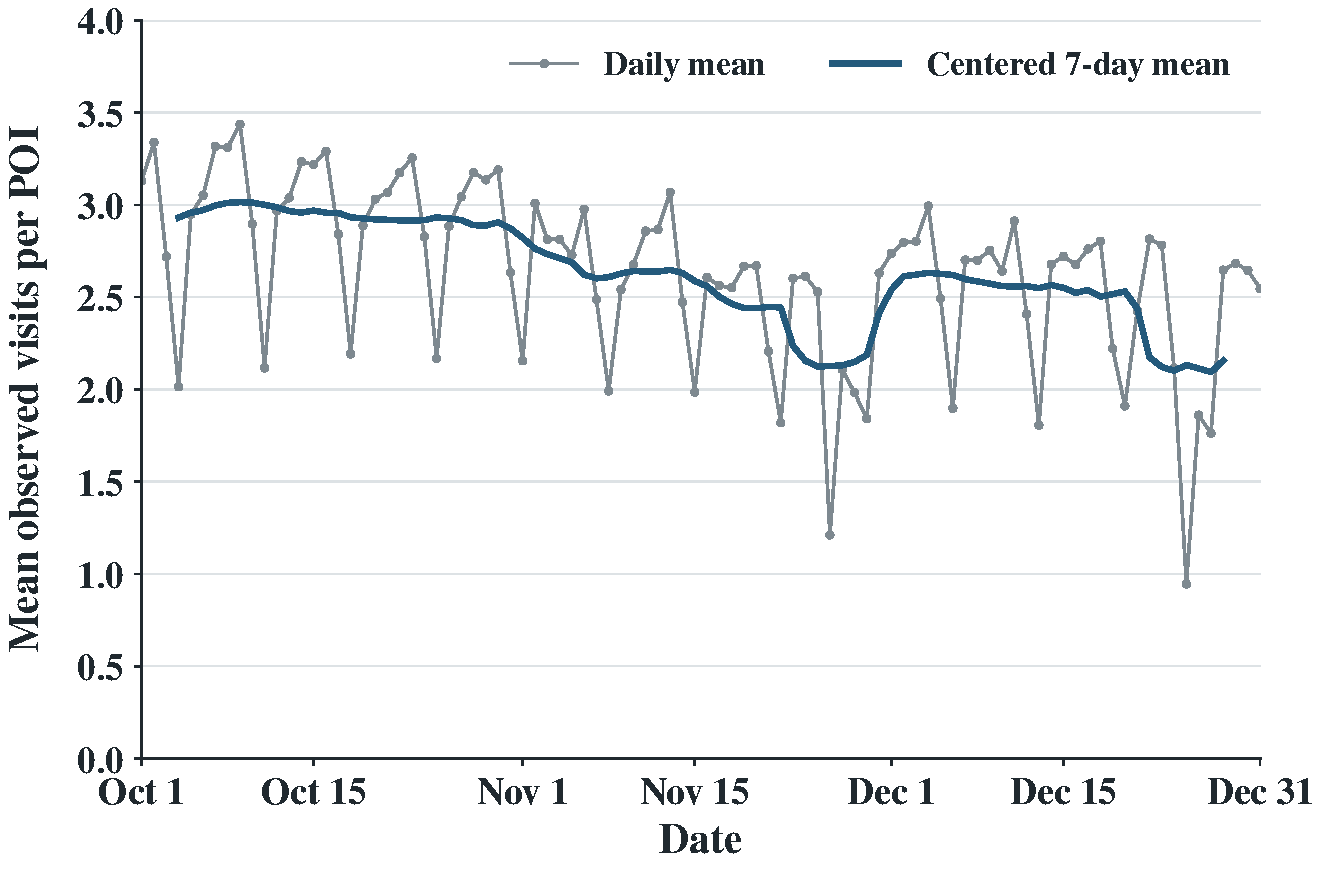
\includegraphics[width=\linewidth]{art/daily_visit.pdf}
    \caption{Daily mean observed visits per POI.}
    \label{fig:daily_visit}
\end{subfigure}
\hfill
\begin{subfigure}[t]{0.49\textwidth}
    \centering
    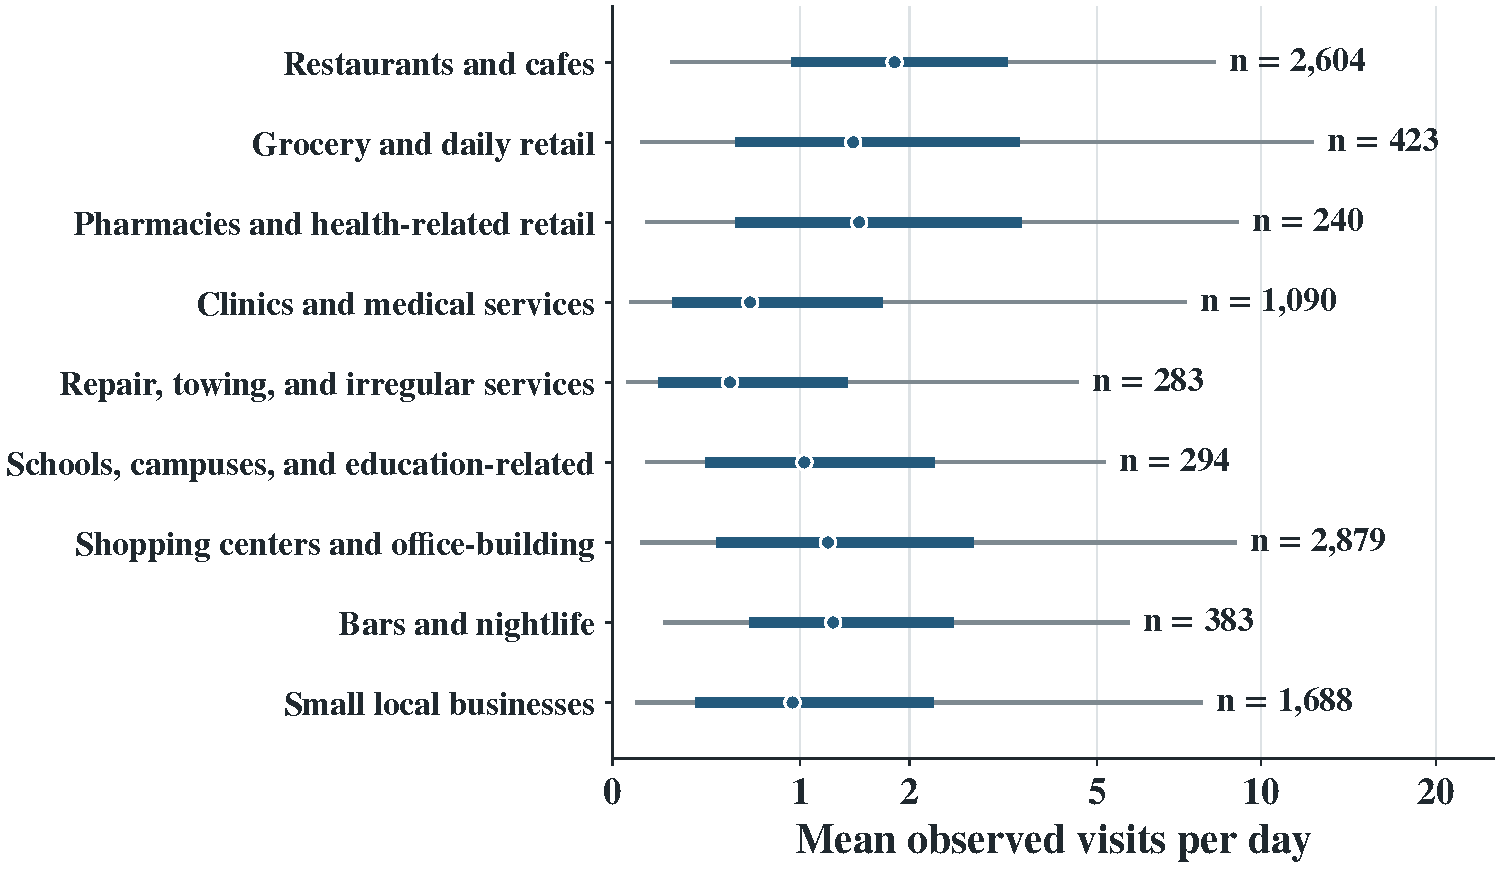
\includegraphics[width=\linewidth]{art/category_visit.pdf}
    \caption{Distribution of mean observed visits across POI categories.}
    \label{fig:category_visit}
\end{subfigure}
\caption{Temporal and category-level characteristics of observed POI visits.}
\label{fig:visit_overview}
\end{figure}

Figure~\ref{fig:visit_overview} summarizes the temporal and category-level variation in observed POI visits.
Panel (a) shows short-term fluctuations and broader temporal changes in aggregate activity, while Panel (b) shows substantial differences in visit levels across the broad POI categories used in the subsequent category-level analysis.

\begin{figure}[!htb]
\centering
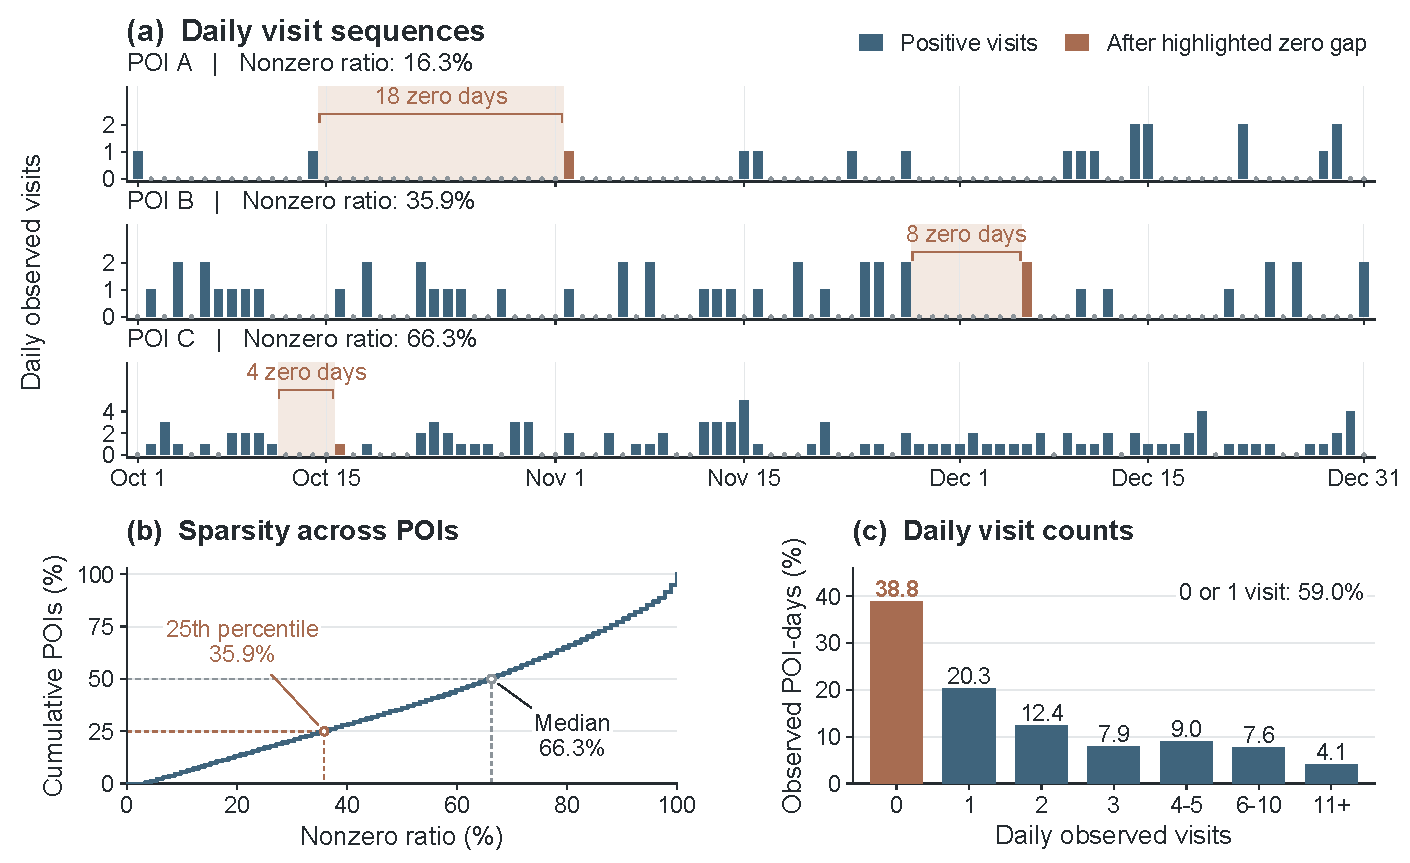
\includegraphics[scale=0.65]{art/poi_temporal_sparsity.pdf}
\caption{Temporal sparsity in POI visit records over the 92-day observation period. (a) Representative daily visit sequences with zero-visit gaps followed by positive visits. (b) Cumulative distribution of POI-level nonzero ratios. (c) Distribution of daily observed visit counts.}
\label{fig:poi_temporal_sparsity}
\end{figure}

Figure~\ref{fig:poi_temporal_sparsity} further shows that POI visits are sparse and intermittent, with prolonged zero-visit periods followed by occasional positive visits.
Across the full observation period, \(38.8\%\) of POI--day observations are zero, and \(59.0\%\) have at most one visit.
The median daily visit count is only \(1\), compared with approximately \(6\), \(9\), and \(22\) visits at the 90th, 95th, and 99th percentiles, respectively.
The maximum daily visit count is substantially larger, producing a long right tail in the visit distribution.
As a result, the data contain a large number of zero or low-count observations together with a much smaller number of high-activity observations.

We then examine POI-level activity to assess whether sparsity is concentrated among particular locations or broadly distributed across POIs.
As shown in Figure~\ref{fig:poi_temporal_sparsity}(b), the median nonzero ratio is \(66.3\%\) over the full observation period, compared with \(35.9\%\) at the 25th percentile.
Over the training period, the corresponding ratios are \(70.0\%\) and \(38.0\%\).
At the lower end of the training-period distribution, \(159\) POIs are active on no more than \(5\%\) of observed days and \(624\) are active on no more than \(10\%\).
Thus, sparsity varies substantially across POIs rather than being uniformly distributed across the visit matrix.
The amount of self-history, namely the historical visit information of a POI, available for forecasting therefore differs considerably across locations, motivating a separate examination of forecasting performance for POIs with limited historical activity.


\subsection{Prediction Task}
\label{subsec:prediction_task}

We first consider the task of forecasting future daily visits for the \(N\) POIs.
For forecast sample \(b\), the model observes visits over the preceding \(T\) days and predicts visits over the following \(H\) days, where \(T\) is the historical input length and \(H\) is the forecast horizon.
The forecasting problem is therefore multistep, with each model producing an \(H\)-day visit trajectory for every POI.

For sample \(b\), the dynamic features consist of historical visit counts \(X_{b,1,t,j}\), where \(X_{b,1,t,j}\) denotes the observed visit count of POI \(j\) at historical step \(t\), with \(t=1,\ldots,T\) and \(j=1,\ldots,N\).
Across all POIs, these features form the historical visit tensor \(\mathbf{X}_b\in\mathbb{R}^{1\times T\times N}\).
In addition, let \(\mathbf{s}_j\in\mathbb{R}^{D_s}\) denote the encoded static-feature vector of POI \(j\), where \(D_s\) is the number of encoded static-feature dimensions.
For the GNN-static formulation, we replicate \(\mathbf{s}_j\) across the \(T\) input steps and concatenate it with the historical visits along the feature dimension.
The resulting augmented input is \(\widetilde{\mathbf{X}}_b\in\mathbb{R}^{(1+D_s)\times T\times N}\).
The observed and predicted future visits are
\(\mathbf{Y}_b=[Y_{b,h,j}]\) and
\(\hat{\mathbf{Y}}_b=[\hat{Y}_{b,h,j}]\), respectively, with
\(\mathbf{Y}_b,\hat{\mathbf{Y}}_b\in\mathbb{R}_{\geq0}^{H\times N}\),
where \(Y_{b,h,j}\) and \(\hat{Y}_{b,h,j}\) denote the observed and predicted visit counts, respectively, for POI \(j\) at forecast lead \(h\) in sample \(b\), with \(h=1,\ldots,H\) and \(j=1,\ldots,N\).
Neural training losses use the raw outputs in visit units. Validation and evaluation replace each output by its maximum with zero; \(\hat{Y}_{b,h,j}\) denotes this nonnegative forecast throughout the metrics, graph-transfer diagnostics, and attribution analysis. Linear baselines use the same truncation.

We compare 14- and 28-day input histories and evaluate each of the seven forecast steps.
A longer historical input contains more weekly cycles, while later forecast steps require predictions further from the observed period.
We further examine whether forecasting performance differs between POIs with frequent positive historical visits and those with sparse or intermittent visit histories.
Locations with frequent positive visits provide more direct evidence of future activity, whereas sparse or intermittent histories may contain predominantly zero observations.
For such POIs, a model can obtain relatively low aggregate error by repeatedly predicting values close to zero while failing to recover occasional positive visits.
We refer to this behavior as \textit{zero-demand collapse}.
Accordingly, we supplement aggregate forecasting metrics with diagnostics for low-history POIs that separately evaluate positive- and zero-visit observations.


\subsection{Attribution Task}
\label{subsec:attribution_task}

The forecasting task provides the predictive model used to estimate future POI visits, which then serves as the basis for examining what information drives each prediction.
We therefore complement the prediction analysis with an attribution task that distinguishes two sources of predictive information: information transferred from related POIs and information associated directly with the target POI.

\subsubsection{Cross-POI Information}

A target POI may receive information from other locations through geographic proximity, functional similarity, or similarity in historical activity. Such information can supplement limited self-history, especially when the target POI has sparse or irregular observations, but it may also overestimate demand when related POIs exhibit activity that is not realized at the target location. 
We refer to the incorporation of related POIs' historical visit information into the prediction for the target POI through graph connections as cross-POI \textit{information transfer}.
For each target POI, forecast lead, and sample, we consider this transfer \textit{beneficial} when it reduces prediction error compared with using only the history of the target POI, and \textit{harmful} when it increases the error.

To capture dependencies across locations, previous studies have used adjacency matrices to represent geographic proximity, functional similarity, and correlations in historical activity \citep{geng2019spatiotemporal,hajisafi2023learning}. Following this approach, we represent relationships among POIs using an adjacency matrix \(A\in\mathbb{R}^{N\times N}\), where \(A_{ij}\) represents the relationship strength from POI \(j\) to POI \(i\). We consider four types of adjacency matrices. The identity matrix contains only self-connections and serves as a baseline without cross-POI information transfer. Spatial matrices capture geographic proximity through nearest-neighbor connections or distance-based weights. Functional matrices represent similarities among POIs based on shared category labels or industry classifications at different levels of detail. Finally, visit-correlation matrices capture similarities in training-period daily visits.

Using the adjacency matrices described above, we adopt a graph neural network with adjacency-based information sharing (GNN-adj) formulation, where the model input \(\mathbf{X}_b\in\mathbb{R}^{1\times T\times N}\) contains only historical visit counts, and the selected adjacency matrix \(A\) controls information propagation across POIs. We first compare forecasting performance under different graph structures against the identity-adjacency baseline. Subsequently, we perturb the historical visits of selected groups of connected POIs to examine their influence on target POI predictions, distinguishing \textit{beneficial} transfer, which reduces prediction error relative to the identity-adjacency baseline, from \textit{harmful} transfer, which increases it.


\subsubsection{Target-POI Information}

The second part of the attribution task examines information associated directly with the target POI. In addition to historical visits, each POI has static attributes describing its location, functional identity, brand, parent-place context, and operating conditions. These attributes may help explain why POIs with similar recent visit histories receive different predictions.


To isolate target-POI information from cross-POI propagation, we use the \textit{GNN-static} formulation with the augmented input \(\widetilde{\mathbf{X}}_b\) and identity adjacency, i.e., \(A=I_N\).
At each forecast origin, this specification uses the history of the target POI and static attributes, with parameters learned jointly across training POIs.
This formulation supports the subsequent \textit{Feature Attribution and POI Regimes} analysis, where gradient-based attribution is used to quantify the contributions of self-history and static POI attributes to individual predictions.
POIs are then compared according to their attribution profiles to examine whether different locations rely on systematically different sources of predictive information.

To examine how different POI relationships affect forecasting, we use \textit{GNN-adj} in \textit{Alternative Adjacency Matrices}, where the historical visit inputs remain fixed while the adjacency matrix varies.
We also use \textit{GNN-adj} in \textit{Related-POI Perturbation Analysis}, as perturbing the historical visits of connected POIs allows us to examine how information transferred through the graph affects target POI predictions.
In contrast, to identify the contributions of the historical visits and static attributes of a target POI, we use \textit{GNN-static} in \textit{Feature Attribution and POI Regimes}, where identity adjacency excludes cross-POI information transfer and allows attribution analysis to focus on target-specific features.

\section{Methodology}
\label{sec:methodology}

To evaluate POI visit forecasting under different temporal and cross-POI dependencies, we first introduce two temporal graph networks, i.e., GraphGRU and MTGNN, alongside the benchmark models.
We then describe alternative adjacency matrices and static POI features to represent relationships among POIs and their individual characteristics.
For POIs with sparse visit histories, we introduce additional evaluation metrics to assess whether the models can capture occasional positive visits without overpredicting activity on days with no observed visits.
Finally, we employ related-POI perturbation analysis and gradient-based feature attribution to investigate the sources of cross-POI information transfer and the factors driving individual predictions.

\subsection{Forecasting Models}
\label{subsec:forecasting_models}
\subsubsection{Benchmark Models}
\label{subsubsec:benchmark_models}
The benchmarks include historical averages, autoregressive ridge regression (AR-ridge), LSTM, NLinear-ridge, and an intermittent-demand model.

\textit{(1) Historical Average.}
The historical-average (HA) predictor uses equally weighted observed training days.
Let \(\mathcal T_{\mathrm{tr}}\) denote the training calendar, \(\mathcal T_{\mathrm{tr},j}\) its dates with an observed count for POI \(j\), and \(y_{\tau,j}\) that count.
Its forecast is \(\bar y_j^{\mathrm{hist}}=|\mathcal T_{\mathrm{tr},j}|^{-1}\sum_{\tau\in\mathcal T_{\mathrm{tr},j}}y_{\tau,j}\).
We also evaluate a same-weekday training mean, the last observation, a repeated last-week forecast, and a recent mean whose window is selected by validation mean absolute error (MAE) from 7, 14, and 28 days subject to the available input length.
These additional benchmarks use the same scored test events as the fitted models.
We fit a ridge-regression implementation of NLinear \citep{zeng2023transformers}, denoted NLinear-ridge, with weights shared across POIs. It subtracts the last observation before the affine forecast and restores that observation afterward; we solve its ridge-regularized squared-error objective directly and select the penalty from \(\{0,10^{-4},10^{-2},1\}\) by validation MAE.
The Teunter--Syntetos--Babai (TSB) benchmark \citep{teunter2011intermittent} separately smooths positive-visit size and visit-occurrence probability, selecting both smoothing constants from \(\{0.05,0.1,0.2\}\) on validation MAE.

\textit{(2) AR-ridge.}
AR-ridge models the linear relationship between historical visits and future demand.
For POI \(j\), let \(\mathbf v_{b,j}\in\mathbb{R}^{T+1}\) contain a leading constant followed by its historical visits in sample \(b\), and let \(\mathbf y_{b,j}\in\mathbb{R}^{H}\) contain its next \(H\) visits.
The model takes the form
\(\mathbf y_{b,j}=B_j^\top\mathbf v_{b,j}+\boldsymbol{\varepsilon}_{b,j}\),
where \(B_j\in\mathbb{R}^{(T+1)\times H}\) is the coefficient matrix and \(\boldsymbol{\varepsilon}_{b,j}\) is the error term.
Ridge regularization penalizes the lag coefficients while leaving the intercept unpenalized; one penalty is selected for all POIs and leads by validation MAE.
This baseline provides a linear reference for assessing how effectively the historical visits of a POI predict future activity.

\textit{(3) LSTM.}
The LSTM baseline \citep{hochreiter1997long} processes historical visit sequences recurrently.
It processes the univariate history of each POI independently, with recurrent weights shared across POIs.
We denote this specification Shared-LSTM.
A decoder maps the final 32-dimensional hidden state to \(H\) forecasts.
This provides a nonlinear temporal reference with the same hidden dimension and training loss as GraphGRU.

A resource probe of the official BysGNN implementation used the full 9,884-POI cohort shape and batch size four. Its per-POI recurrent units contain 979 million parameters, and the attention forward pass exhausted the 23.52-GiB GPU memory. The reproducibility archive retains the source hash and allocation trace.

\subsubsection{GraphGRU}
\label{subsubsec:evolvegcn}
GraphGRU applies a fixed graph operator to historical visits, projects the inputs for each POI to 32 dimensions, and processes the sequence with a shared gated recurrent unit (GRU).
For functional graphs, the propagated input is the average of the target count and its group mean, including the target in that mean.
The decoder combines the final recurrent state with a linear projection of the last observation of the target POI to produce \(H\) forecasts.
The graph operator is fixed; the recurrent state evolves across input days.

The GNN-static specification uses this same recurrence with identity adjacency and adds static attributes to the input projection at each time step.
Its 52 static dimensions comprise four numeric inputs and six learned eight-dimensional embeddings for category, NAICS-2, NAICS-4, brand, parent place, and sub-category.
The numeric inputs are latitude, longitude, opening hours, and an opening-hour missingness indicator.
We standardize these four inputs across POIs with observed training visits and retain those transformations for validation and testing.
Brand and parent-place labels appearing at most 20 times are pooled; missing labels form a separate category. Other categorical labels appearing only once are pooled.

\subsubsection{MTGNN}
\label{subsubsec:mtgnn}

MTGNN combines temporal convolution with graph learning for multivariate time-series forecasting \citep{wu2020connecting}.
A central motivation of MTGNN is that the true dependency structure among variables may not be fully observed in advance.
The model therefore includes an adaptive graph-learning component together with temporal convolutions that capture lagged dependence.

The fixed MTGNN specification, denoted Fixed-MTGNN, disables graph learning and holds the supplied adjacency fixed.
Both graph-propagation directions use the selected relation, while temporal convolutions model lagged dependence.
For functional graphs, propagation averages the current node representation with its group mean; identity adjacency leaves it unchanged.
For sampled, spatial, and visit-correlation graphs, we first normalize the supplied adjacency by rows.
The two propagation directions use this matrix and its transpose, respectively, adding self-connections and renormalizing rows within each direction.
The implementation normalizes across channels and time within each node, with POI-specific learned affine parameters; identity adjacency therefore does not mix POI histories through normalization.
The adaptive specification, denoted Adaptive-MTGNN, learns a directed top-20 graph from node embeddings.
Its candidate scores are evaluated in blocks, and gradients are retained for the selected edge weights; this implements the same top-\(k\) graph operator without storing a dense adjacency gradient.
Tie-breaking noise is fixed during validation and testing.
Both specifications use the same temporal architecture and within-POI normalization.

\subsection{Adjacency Matrices}
\label{subsec:adjacency}

To examine how different relationships among POIs affect forecasting performance, we consider four types of adjacency matrices: \textit{identity adjacency}, \textit{spatial adjacency}, \textit{functional adjacency}, and \textit{visit-correlation adjacency}.

\textit{(1) Identity Adjacency.}
The identity adjacency, \(A=I_N\), contains only self-connections.
It excludes cross-POI information transfer while preserving the information of each POI.

\textit{(2) Spatial Adjacency.}
Spatial relationships are represented using two types of graphs: \(k\)-nearest neighbors (KNN) \citep{cover1967nearest} and radial basis function (RBF) \citep{li2018diffusion}.
The KNN graph connects each POI to its \(k\) geographically nearest locations and takes the symmetric union of these connections.
The RBF graph instead assigns continuous distance-decay weights,
\(A_{ij}=\exp[-d(i,j)^2/(2\sigma^2)]\mathbb{I}\{d(i,j)\leq2\text{ km}\}\) for \(i\ne j\),
where \(A_{ij}\) denotes the relationship strength from POI \(j\) to POI \(i\), \(d(i,j)\) is their geographic distance, \(\sigma=1\text{ km}\) controls distance decay, and \(\mathbb{I}\{\cdot\}\) equals one when its condition holds and zero otherwise. We set the diagonal to one and normalize each row before constructing the model-specific propagation operators described above.

\textit{(3) Functional Adjacency.}
Functional relationships are represented using NAICS-2 and NAICS-4.
For each classification \(q\in\{\mathrm{naics2},\mathrm{naics4}\}\), the corresponding adjacency matrix is defined as
\(
A_{ij}^{(q)}=\mathbb{I}\{q_i=q_j\},
\)
where \(q_i\) and \(q_j\) denote the classification labels or industry-code prefixes of POIs \(i\) and \(j\), respectively.
NAICS-2 represents broader functional groups, whereas NAICS-4 represents more specific classifications.
Top category produces the same graph as NAICS-4 in this cohort.
To separate semantic grouping from neighborhood size, we also sample NAICS-2, NAICS-4, and random neighbors with identical non-self row degrees.
Each target receives the smaller of \(k\) and its number of NAICS-4 peers, with \(k\in\{5,10,20\}\); singleton NAICS-4 groups remain isolated in all three controls.
GraphGRU averages the normalized neighbor signal with the input of the target POI, and isolated rows retain the target input.
The sampled controls match row degrees; the transposed MTGNN operator also reflects column-degree variation.

\textit{(4) Visit-Correlation Adjacency.}
Historical similarity is represented using Pearson correlations between POI visit sequences.
Specifically, the correlation between POIs \(i\) and \(j\) is computed as
\(\rho_{ij}=\operatorname{corr}((y_{\tau,i})_{\tau\in\mathcal{T}_{\mathrm{tr}}},(y_{\tau,j})_{\tau\in\mathcal{T}_{\mathrm{tr}}})\),
where \(\operatorname{corr}(\cdot,\cdot)\) denotes the Pearson correlation coefficient computed from the daily visit counts of the two POIs over the training period.
For the static correlation graph, the adjacency weights are defined as
\(A_{ij}=|\rho_{ij}|\mathbb{I}\{|\rho_{ij}|\geq\eta_c\}\),
where \(\eta_c\) is the threshold used to remove weak correlations.
All reported visit-correlation graphs use training-period observations and remain fixed during validation and testing.

\subsection{Forecast Evaluation}
\label{subsec:low_history_method}

We evaluate overall forecasting accuracy, visit-density sensitivity, low-history POI behavior, and the coverage of observed activity under spatial prioritization.

\textit{(1) Overall Forecasting Accuracy.}
We evaluate forecasting accuracy using MAE and root mean squared error (RMSE).
MAE measures average absolute error, while RMSE gives greater weight to large errors.
MAE skill relative to HA is \(100(1-\mathrm{MAE}^{\mathrm{model}}/\mathrm{MAE}^{\mathrm{HA}})\).
Metrics pool scored events across forecast origins, leads, and POIs within each setting.
Forecast windows overlap, so the same observed POI-day can be predicted at several leads from different origins.

\textit{(2) Visit-Density Sensitivity.}
To examine how historical visit sparsity affects forecasting performance, we construct POI subsets with progressively higher frequencies of positive visits.
For POI \(j\), the training-period nonzero ratio is defined as
\(
r_j=
\frac{1}{|\mathcal{T}_{\mathrm{tr},j}|}
\sum_{\tau\in\mathcal{T}_{\mathrm{tr},j}}
\mathbb{I}\{y_{\tau,j}>0\}.
\)
We consider three approaches to constructing these subsets.
The \textit{density-based} approach ranks POIs by their training-period nonzero ratios \(r_j\).
The \textit{recent-density} approach ranks POIs by their nonzero ratios over the final \(L_{\mathrm{rec}}\) days of the training period, where \(L_{\mathrm{rec}}\) denotes the recent-history window length.
The \textit{persistence-density} approach ranks POIs by the product of the overall nonzero ratio and the probability of consecutive positive-visit days, estimated as \(p_j^{\mathrm{persist}}=\frac{\sum_{\tau\in\mathcal{T}_{\mathrm{tr},j}^{-}}\mathbb{I}\{y_{\tau,j}>0,\;y_{\tau+1,j}>0\}}{\sum_{\tau\in\mathcal{T}_{\mathrm{tr},j}^{-}}\mathbb{I}\{y_{\tau,j}>0\}}\), where \(\mathcal{T}_{\mathrm{tr},j}^{-}\) contains training days with both the current and following count observed for POI \(j\); the probability is zero when its denominator is zero.
For each approach, we exclude the lowest-ranked fraction, denoted by \(\gamma^{\mathrm{den}},\gamma^{\mathrm{rec}},\gamma^{\mathrm{per}}\in(0,1)\), respectively, breaking tied scores by the fixed POI order.
We consider quantile thresholds of \(0.10\), \(0.25\), \(0.50\), and \(0.75\), corresponding to the percentages of POIs excluded from each subset.
For example, Dense10 retains the top \(90\%\) of POIs ranked by their training-period nonzero ratios.
The same suffix convention applies to the recent-density and persistence-density subsets.
For each subset, we reconstruct the visit matrix and retrain the forecasting model.

\textit{(3) Low-History POI Evaluation.}
To assess forecasting performance for POIs with sparse historical activity, we identify locations characterized by frequent zero observations and low average visit counts.
The low-history POI set is defined as
\(\mathcal{I}_{0}=\left\{j:z_j\geq\eta_z,\;0<\bar y_j^{\mathrm{hist}}\leq Q_{\alpha}\right\}\),
where \(z_j=|\mathcal T_{\mathrm{tr},j}|^{-1}\sum_{\tau\in\mathcal T_{\mathrm{tr},j}}\mathbb I\{y_{\tau,j}=0\}\) is the zero-visit ratio over observed training days, and \(Q_{\alpha}\) is the \(\alpha\)-quantile of strictly positive historical averages across POIs.
Using the first 50 calendar days for identification fixes the same 1,944-POI cohort across input lengths, models, seeds, and evaluation months.
For these POIs, we distinguish test events with positive observed visits from those with zero observed visits, defined respectively as
\(\Omega_0^+=\{(b,h,j):j\in\mathcal{I}_0,\;Y_{b,h,j}>0\}\)
and
\(\Omega_0^0=\{(b,h,j):j\in\mathcal{I}_0,\;Y_{b,h,j}=0\}\).
We evaluate forecast magnitude on positive events and distinguish positive-event detection from false activation.

\textit{(i) Demand Mass Recovery Ratio (DMR).}
DMR measures the ratio of predicted to observed visit totals among events with positive realized demand,
i.e., 
\(\mathrm{DMR}^{\mathrm{model}}=\frac{\sum_{(b,h,j)\in\Omega_0^+}\hat Y_{b,h,j}}{\sum_{(b,h,j)\in\Omega_0^+}Y_{b,h,j}}\),
while the corresponding HA baseline is
\(\mathrm{DMR}^{\mathrm{HA}}=\frac{\sum_{(b,h,j)\in\Omega_0^+}\bar y_j^{\mathrm{hist}}}{\sum_{(b,h,j)\in\Omega_0^+}Y_{b,h,j}}\).
The difference
\(\Delta\mathrm{DMR}=\mathrm{DMR}^{\mathrm{model}}-\mathrm{DMR}^{\mathrm{HA}}\)
measures the change in predicted demand mass relative to the HA baseline.

\textit{(ii) False Activation Rate (FAR).}
FAR measures the proportion of zero-visit events for which the predicted visit count reaches a specified threshold.
For an activation threshold \(\eta_{\mathrm{FAR}}>0\), we define
\(\mathrm{FAR}_{\eta_{\mathrm{FAR}}}=\frac{1}{|\Omega_0^0|}\sum_{(b,h,j)\in\Omega_0^0}\mathbb{I}\{\hat Y_{b,h,j}\geq\eta_{\mathrm{FAR}}\}\).
We also report recall, precision, and average precision (AP) for detecting positive visits, using activation thresholds of \(0.1,0.25,0.5,1,2\) visits.
Recall is the activated fraction of positive events, precision is the positive fraction of activated events, and AP integrates precision over increases in recall while treating tied scores as one threshold.
To separate forecast scale from event discrimination, we fit the calibration \(\max\{0,a\hat Y_{b,h,j}+c\}\) on low-history validation events only.
The slope \(a\) lies in \([0,20]\), and the absolute intercept \(|c|\) is bounded by the larger of one and the 99th percentile of their observed visits.
We use bounded Powell search with validation MAE as the objective and retain the identity transformation as a candidate.
For each model, we additionally choose thresholds that keep validation FAR at or below \(5\%,10\%,20\%,30\%\), then report recall and realized FAR on the test events.

\textit{(4) Spatial Activity Prioritization.}
To assess whether forecast accuracy translates into identifying areas with high observed activity, we partition the cohort into fixed 1-km grid cells and rank their summed POI forecasts for each origin and lead.
We select the highest-ranked \(K\) cells, where \(K\) is the rounded-up number corresponding to \(5\%,10\%,20\%\) of occupied cells.
Let \(S_{b,h}\) denote the POIs in those selected cells for sample \(b\) and lead \(h\).
Coverage is the fraction of observed visits in the selected cells, i.e.,
\[
\mathrm{Coverage}_{b,h}
=\frac{\sum_{j\in S_{b,h}}Y_{b,h,j}}{\sum_{j=1}^{N}Y_{b,h,j}}.
\]
We average coverage over forecast origins and leads and compare it with the retrospective upper bound obtained by ranking cells using observed visits.
This experiment evaluates the prioritization of observed location-level activity under a fixed monitoring budget.

\subsection{Related-POI Perturbation Analysis}
\label{subsec:perturbation_method}

Building on the low-history POI evaluation, we further examine how information transferred from related POIs affects individual predictions.
We first identify \textit{graph-transfer regimes} based on graph lift and historical activity at the target and neighboring POIs, and then conduct \textit{neighbor-group perturbation} to identify which neighbors contribute to the observed prediction changes.

\textit{(1) Graph-Transfer Regimes.}
We characterize cross-POI information transfer by comparing predictions from the same forecasting architecture under different adjacency matrices.
For test sample \(b\), forecast lead \(h\), and target POI \(j\), let \(\hat Y_{b,h,j}^{A}\) denote the prediction under a non-identity adjacency matrix \(A\), and \(\hat Y_{b,h,j}^{\mathrm{ID}}\) the corresponding prediction under identity adjacency.
Their difference, defined as
\(G_{b,h,j}=\hat Y_{b,h,j}^{A}-\hat Y_{b,h,j}^{\mathrm{ID}}\),
is termed \textit{graph lift}. The two models are fitted separately, so this contrast includes changes in learned parameters as well as adjacency. The subsequent fixed-model perturbations isolate sensitivity to neighbor inputs.

For low-history POIs \(j\in\mathcal{I}_0\), we characterize graph transfer using the historical activity of the target POI and its connected neighbors.
Let \(\mathcal{N}(j)=\{i\neq j:A_{ji}>0\}\) denote the neighbors of POI \(j\) under the selected adjacency matrix.
We define \textit{target evidence} as the average historical visits of the target POI,
\(\frac{1}{T}\sum_{t=1}^{T}X_{b,1,t,j}\),
and \textit{neighbor evidence} as the average historical visits across its connected neighbors,
\(\frac{1}{T|\mathcal{N}(j)|}\sum_{i\in\mathcal{N}(j)}\sum_{t=1}^{T}X_{b,1,t,i}\),
for POIs with nonempty neighborhoods.
Under functional adjacency, neighbor evidence summarizes historical activity among POIs sharing the corresponding functional classification.

We classify prediction events according to target evidence, neighbor evidence, graph lift, and realized visits.
Low and high levels of target and neighbor evidence are determined using their respective empirical medians among low-history validation events.
Positive graph lift is defined by \(G_{b,h,j}\geq\eta_G\), where \(\eta_G>0\) is the graph-lift threshold.
Positive activation follows the threshold \(\eta_{\mathrm{FAR}}\) defined in the preceding subsection.
Table~\ref{tab:graph_transfer_regime_definitions} summarizes the resulting graph-transfer regimes. Events are assigned in the order spurious, substitutive, confirmatory, redundant, and conservative zero; unassigned events form Other. Because realized visits enter these definitions, the regimes describe forecast outcomes after observation.

\begin{table}[t]
\centering
\begin{adjustbox}{max width=\textwidth}
\begin{tabular}{lll}
\toprule
Regime & Definition & Interpretation \\
\midrule
Substitutive transfer
& Low target evidence, high neighbor evidence, positive graph lift
& Neighbor activity supplements limited target history. \\
Spurious transfer
& Substitutive transfer with \(Y_{b,h,j}=0\) and positive activation
& Neighbor information raises predictions for zero-visit events. \\
Confirmatory transfer
& High target evidence, high neighbor evidence, positive graph lift
& Neighbor activity reinforces target-history information. \\
Redundant self-history
& High target evidence, small or negative graph lift
& Predictions rely primarily on target-history information. \\
Conservative zero
& \(Y_{b,h,j}=0\) and no positive activation
& The model maintains low predictions for zero-visit events. \\
\bottomrule
\end{tabular}
\end{adjustbox}
\caption{Graph-transfer regime definitions for low-history POIs.}
\label{tab:graph_transfer_regime_definitions}
\end{table}

To assess the predictive value of graph transfer, we compute the event-level MAE gain as
\(|Y_{b,h,j}-\hat Y_{b,h,j}^{\mathrm{ID}}|-|Y_{b,h,j}-\hat Y_{b,h,j}^{A}|\).
Positive values indicate lower prediction error under non-identity adjacency, whereas negative values indicate higher error.
We compare graph lift and MAE gain across the identified regimes to characterize the conditions under which cross-POI information improves or worsens forecasting accuracy.
We separately report MAE gain in the four low/high target-evidence and neighbor-evidence strata, whose membership uses only the inputs available at the forecast origin.

\textit{(2) Neighbor-Group Perturbation.}
We further examine which neighboring POIs contribute to the graph-transfer effects identified above.
For each target POI \(j\), we select a group \(S\subseteq\mathcal{N}(j)\) and perturb its historical visit inputs while keeping the forecasting model and adjacency matrix fixed.
Let \(\mathbf{X}_b^{(-S)}\) denote the input obtained by setting the historical visits of POIs in \(S\) to zero while leaving all other inputs unchanged.
The perturbation effect is defined as
\begin{equation}
D_{b,h,j}(S)
=
\hat Y_{b,h,j}^{A}(\mathbf{X}_b)
-
\hat Y_{b,h,j}^{A}(\mathbf{X}_b^{(-S)}),
\label{eq:perturbation_effect}
\end{equation}
where a positive value indicates that the selected neighbor group increases the original prediction for the target POI.

We compare neighbors selected by training-period mean activity, pairwise observed training correlation, activity during the final seven input days, and uniform random sampling.
Every rule perturbs the same number of neighbors for a given target, equal to the smaller of ten and its number of NAICS-4 peers, under both NAICS-2 and NAICS-4.
The target set consists of the 1,935 low-history POIs with at least one NAICS-4 peer.
An additional intervention replaces the most active neighbors' histories with histories from outside the functional group, matched on training-standardized log mean, nonzero frequency, and log standard deviation.
Perturbing disconnected nodes provides a negative control.
We evaluate forecast changes and MAE changes on identical events, including the evidence strata defined above.

\subsection{Feature Attribution and POI Regimes}
\label{subsec:attribution_method}

The preceding analysis examines the influence of information transferred through graph connections.
We next investigate the contributions of the historical visits and static attributes of a target POI using the GNN-static formulation introduced in Section~\ref{subsec:attribution_task}.
With identity adjacency excluding cross-POI propagation, we apply gradient-based attribution to individual predictions and examine how the resulting information sources vary across POIs.

\textit{(1) Gradient-Based Feature Attribution.}
We use Gradient \(\times\) Input to quantify the contribution of each input component to an individual prediction.
Let \(x_{b,j,m}\), \(m=1,\ldots,T+D_s\), index the \(T\) historical visits followed by the \(D_s\) encoded static components of POI \(j\). Each static component is shared across input steps, so its derivative sums the effects through all \(T\) copies in \(\widetilde{\mathbf{X}}_b\).
The attribution score for forecast lead \(h\) is defined as
\(\phi_{b,h,j,m}=x_{b,j,m}\frac{\partial\hat Y_{b,h,j}}{\partial x_{b,j,m}}\).
The score combines the standardized numeric input or learned embedding component with local prediction sensitivity. Outputs clipped from negative values contribute zero gradient attribution.
We compare it with integrated gradients (IG) \citep{pmlr-v70-sundararajan17a}, which attributes the change from a reference input \(\mathbf x'\) to the observed input \(\mathbf x_{b,j}\), i.e.,
\[
\phi^{\mathrm{IG}}_{b,h,j,m}
=(x_{b,j,m}-x'_m)\int_0^1
\frac{\partial\hat Y_{b,h,j}(\mathbf x'+u(\mathbf x_{b,j}-\mathbf x'))}{\partial x_m}\,\mathrm du.
\]
Here \(u\) indexes the interpolation path.
Two observed POI records define the reference endpoints, selected near the lower and upper quartiles of positive training mean visits and then near the geographic median.
Each endpoint combines the final training-history window of that POI with its complete static record; categorical paths interpolate between learned embeddings.
We use identical sampled events for the method comparison and check that summed signed IG values recover the change in forecast from the reference endpoint.

To summarize attribution across different information sources, we consider five feature groups: \textit{history}, \textit{location}, \textit{identity}, \textit{parent}, and \textit{others}.
History includes historical visit counts; location includes latitude and longitude; identity includes category, industry, and brand information; parent includes parent-place information; and others includes opening-hour features and their missingness indicators.
The parent encoding includes a learned missing-parent category, so its attribution can also be nonzero for POIs without a recorded containing place.
Let \(\mathcal{G}\) denote the set of these groups and \(\mathcal{F}_g\) the input components belonging to group \(g\in\mathcal{G}\).
For fitted seed \(s\in\{42,\ldots,46\}\), let \(\phi^{(s)}_{b,h,j,m}\) denote the corresponding attribution score. We aggregate absolute scores across test samples and forecast leads to obtain the seed-specific share
\begin{equation}
\pi^{(s)}_{j,g}
=
\frac{
\sum_{b,h}
\sum_{m\in\mathcal{F}_g}
|\phi^{(s)}_{b,h,j,m}|
}{
\sum_{g'\in\mathcal{G}}
\sum_{b,h}
\sum_{m\in\mathcal{F}_{g'}}
|\phi^{(s)}_{b,h,j,m}|
}.
\label{eq:attribution_group_share}
\end{equation}
Let \(\mathcal S_j\) contain the fitted seeds with positive total attribution for POI \(j\). We average their shares, \(\pi_{j,g}=|\mathcal S_j|^{-1}\sum_{s\in\mathcal S_j}\pi^{(s)}_{j,g}\). The resulting attribution profile
\(\boldsymbol{\pi}_j=(\pi_{j,g})_{g\in\mathcal{G}}\)
summarizes the relative contributions of different information sources to predictions for POI \(j\).
POIs with zero total attribution remain unassigned.

\textit{(2) Attribution-Based POI Regimes.}
We characterize differences in feature reliance by standardizing these seed-averaged shares across eligible POIs.
For each feature group \(g\in\mathcal{G}\), let \(\mu_g\) and \(\sigma_g\) denote the mean and standard deviation of \(\pi_{j,g}\) across POIs, respectively.
The standardized attribution score is defined as
\begin{equation}
\widetilde{\pi}_{j,g}
=
\frac{\pi_{j,g}-\mu_g}{\sigma_g}.
\end{equation}
Each POI is assigned to the regime corresponding to its highest standardized attribution score.
The resulting five regimes are history-driven, location-driven, identity-driven, parent-driven, and others-driven.
These assignments reflect relative feature reliance across POIs rather than the largest original attribution share.
We further compare forecasting errors across the resulting regimes.
Retraining after removing location, identity, parent, or other static inputs, and after removing all static inputs, measures the predictive contribution of each source separately from its attribution share.

\textit{(3) Parent-Place Attribution.}
To examine the role of containment relationships in POI predictions, we focus on locations with valid parent-place information.
For each embedded POI, we compare the parent-place attribution share \(\pi_{j,\mathrm{parent}}\) with the combined share of the remaining information sources, \(1-\pi_{j,\mathrm{parent}}\).
We then aggregate these shares across different embedded POI groups to assess how reliance on parent-place context varies with POI function and surrounding destination type.
We compare the full and parent-removed fits on the same embedded POIs and relate the parent attribution share of each POI to its change in MAE after removal.

\textit{(4) Semantic Granularity.}
We further examine how category and industry representations at different levels of granularity contribute to individual predictions.
Using GNN-static with identity adjacency, we compare the attribution of four semantic descriptors: top category, sub-category, NAICS-2, and NAICS-4.
For each prediction event, we compute the Gradient \(\times\) Input attribution scores associated with each descriptor and compare their relative contributions.
We report the attribution share of each descriptor and fit four variants retaining one semantic descriptor at a time, while holding the remaining nonsemantic inputs fixed.
The joint specification and additional fits without NAICS-2 or without NAICS-4 assess whether a descriptor adds predictive information when the overlapping classifications are available.

\section{Empirical Results}
\label{sec:results}

Figure~\ref{fig:exp_logic} outlines the empirical analyses, organized into prediction and attribution tasks.
We begin in Section~\ref{subsec:forecasting_results} by comparing forecasting performance across historical input lengths and forecast leads, examining visit-history sparsity, and evaluating positive-demand recovery and false activation for low-history POIs.
To investigate information sharing among POIs, Section~\ref{subsec:information_sharing_results} compares alternative adjacency matrices and examines how related-POI perturbation affects individual forecasts.
Finally, Section~\ref{subsec:explanation_results} analyzes attribution patterns and POI attribution regimes to identify the information sources driving predictions, while examining parent-place context and semantic granularity to assess their roles in forecasting.

\begin{figure}[htbp]
\centering
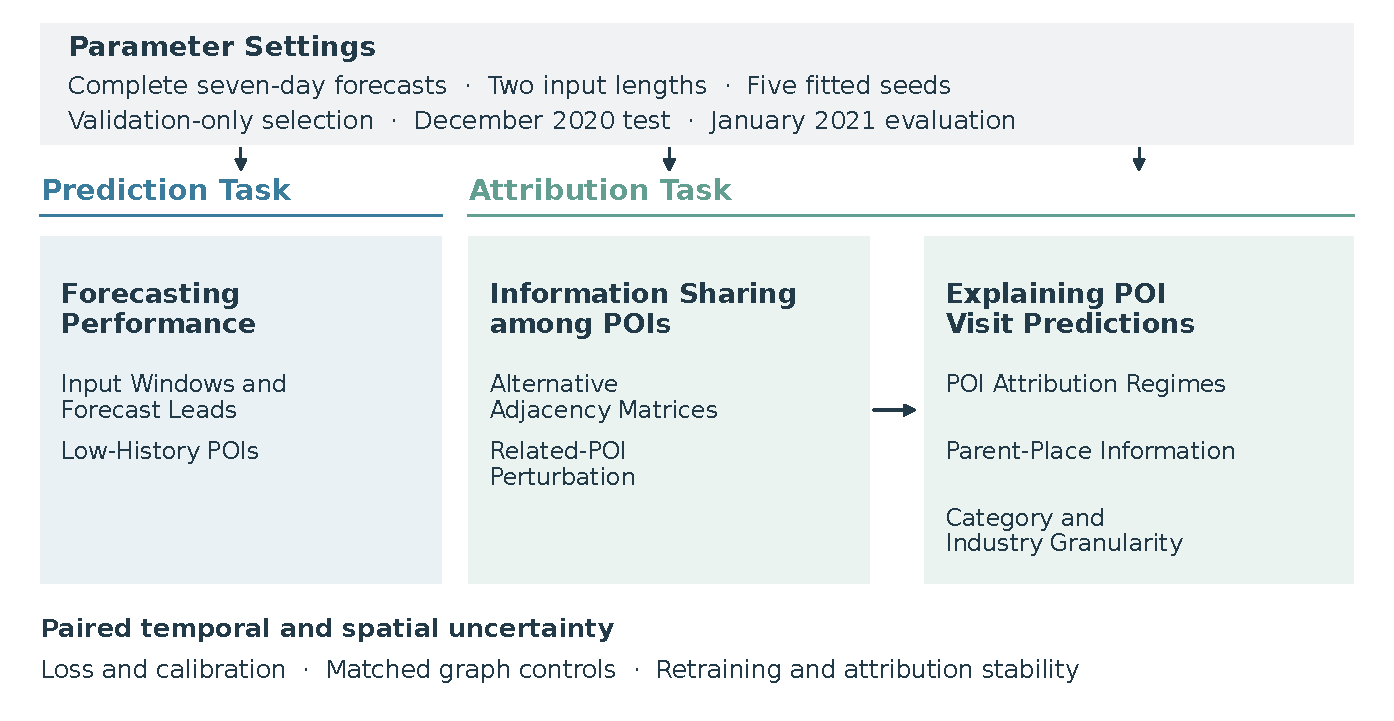
\includegraphics[scale=0.65]{art/exp_logic.pdf}
\caption{Design logic of the empirical analyses.}
\label{fig:exp_logic}
\end{figure}

\subsection{Parameter Settings}
\label{subsec:parameter_settings}

We evaluate \((T,H)\in\{(14,7),(28,7)\}\), retaining only windows whose entire target sequence lies within one split.
Training targets end on November 19, validation targets span November 20--December 3, and December test targets span December 4--31, 2020.
Every forecast lead is therefore represented in validation.
Density sensitivity uses \(T=28\); graph controls, neighbor perturbations, and feature attribution use \(T=14\).
Neural visit normalization uses observed counts from the first 50 calendar days; missing lag values enter as zero placeholders and missing labels are unscored.
The fitted weights, graph parameters, normalization, calibration, and activation thresholds are then held fixed for January 2021, using only observations before each forecast origin as inputs.
\ref{app:checkpoint_replay} documents checkpoint replay and numerical verification.
Table~\ref{tab:revision_protocol} reports the origin counts, and Table~\ref{tab:parameter_settings} in \ref{app:implementation_settings} summarizes the settings.

All neural models minimize masked absolute error in the main comparison.
For each configuration, we select the learning rate by validation MAE at seed 42, retain that fitted model, and repeat the selected configuration at seeds 43--46.
We report means and standard deviations across all five seeds; GraphGRU, MTGNN, and LSTM are also refitted with mean squared error (MSE) loss to examine loss-function sensitivity.
Degree-controlled graph sampling uses the corresponding training seed.
Checkpoints minimize validation MAE, with at most 100 epochs and early stopping after ten epochs without improvement.
Paired error differences use 2,000 seven-origin block resamples, retaining all POIs and leads together, with percentile intervals at 95\% confidence.
Occupied spatial cells of 1, 3, and 5 km provide separate and joint resampling sensitivities.
These intervals describe variation within the observed Seattle panel, conditional on the fitted seeds.
Feature attribution uses eight evenly spaced test origins and all seven leads.
Gradient \(\times\) Input covers all POIs, while its comparison with IG uses a fixed uniform sample of 1,024 POIs across seeds and methods.
\begin{table}[!htbp]
\centering\small
\caption{Forecast origins with complete target windows. Target dates are disjoint across splits, and all seven leads enter validation. January forecasts use the original fitted parameters.}
\label{tab:revision_protocol}
\begin{tabular}{lrrrr}
\toprule
\((T,H)\) & Training & Validation & December & January \\
\midrule
(14,7) & 30 & 8 & 22 & 25 \\
(28,7) & 16 & 8 & 22 & 25 \\
\bottomrule
\end{tabular}
\end{table}




\subsection{Forecasting Performance}
\label{subsec:forecasting_results}


\subsubsection{Input Windows and Forecast Leads}
\label{subsubsec:multi_horizon_results}

We compare input histories of 14 and 28 days for a seven-day forecast window. Table~\ref{tab:multihorizon} reports December performance and the January evaluation using frozen parameters.

\begin{table}[!htbp]
\centering
\begingroup
\singlespacing
\fontsize{9pt}{10.5pt}\selectfont
\setlength{\tabcolsep}{4pt}
\renewcommand{\arraystretch}{1.08}
\caption{MAE for seven-day forecasts. Every December configuration uses 1,522,136 events from 22 origins, and every January configuration uses 1,729,700 events from 25 origins. Neural values are means and standard deviations over all five seeds; deterministic baselines have one value. January retains the original fitted weights and validation choices.}
\label{tab:multihorizon}
\begin{adjustbox}{max width=\linewidth}
\begin{tabular}{lrrrr}
\toprule
Model / adjacency & Dec., $T=14$ & Dec., $T=28$ & Jan., $T=14$ & Jan., $T=28$ \\
\midrule
Historical average & 1.483 & 1.483 & 1.590 & 1.590 \\
Weekday historical average & 1.439 & 1.439 & 1.509 & 1.509 \\
Seasonal naive & 1.484 & 1.484 & 1.452 & 1.452 \\
Recent mean & 1.351 & 1.351 & 1.335 & 1.335 \\
AR-ridge & 1.453 & 1.448 & 1.583 & 1.579 \\
NLinear-ridge & 1.273 & 1.223 & 1.263 & 1.239 \\
TSB & 1.337 & 1.337 & 1.327 & 1.327 \\
Shared-LSTM & $1.360\pm 0.013$ & $1.366\pm 0.009$ & $1.366\pm 0.012$ & $1.384\pm 0.007$ \\
GraphGRU, Identity & $1.302\pm 0.007$ & $1.304\pm 0.008$ & $1.311\pm 0.007$ & $1.327\pm 0.006$ \\
GraphGRU, NAICS-2 & $1.336\pm 0.007$ & $1.338\pm 0.012$ & $1.351\pm 0.010$ & $1.363\pm 0.010$ \\
GraphGRU, NAICS-4 & $1.350\pm 0.004$ & $1.343\pm 0.004$ & $1.361\pm 0.007$ & $1.364\pm 0.004$ \\
Fixed-MTGNN, Identity & $1.227\pm 0.005$ & $1.207\pm 0.005$ & $1.247\pm 0.004$ & $1.250\pm 0.004$ \\
Fixed-MTGNN, NAICS-2 & $1.222\pm 0.008$ & $1.202\pm 0.001$ & $1.244\pm 0.011$ & $1.247\pm 0.003$ \\
Fixed-MTGNN, NAICS-4 & $1.222\pm 0.007$ & $1.208\pm 0.004$ & $1.247\pm 0.011$ & $1.252\pm 0.003$ \\
Adaptive-MTGNN & $1.221\pm 0.007$ & $1.207\pm 0.008$ & $1.240\pm 0.007$ & $1.249\pm 0.008$ \\
GNN-static & $1.301\pm 0.008$ & $1.317\pm 0.038$ & $1.310\pm 0.007$ & $1.339\pm 0.033$ \\
\bottomrule
\end{tabular}
\end{adjustbox}
\endgroup
\end{table}


At $T=14$, Fixed-MTGNN with identity adjacency has December MAE $1.227\pm0.005$, compared with $1.273$ for NLinear-ridge and $1.302\pm0.007$ for GraphGRU with identity adjacency. The corresponding Fixed-MTGNN values for NAICS-2 and NAICS-4 are $1.222\pm0.008$ and $1.222\pm0.007$. GraphGRU with identity adjacency has lower aggregate MAE than either semantic graph at both input lengths.

Extending the input history reduces December MAE from $1.227$ to $1.207$ for Fixed-MTGNN with identity adjacency and from $1.273$ to $1.223$ for NLinear-ridge. GraphGRU with identity adjacency changes from $1.302$ to $1.304$. In January at $T=28$, NLinear-ridge has MAE $1.239$, compared with $1.250$ for Fixed-MTGNN with identity adjacency. Model rankings therefore depend on the evaluation month and input length.

Adaptive-MTGNN attains December MAE $1.221$ at $T=14$ and $1.207$ at $T=28$, close to the corresponding fixed-graph specifications. Its January values are $1.240$ and $1.249$. Figure~\ref{fig:complete_horizon_skill} shows performance at each forecast lead, while Table~\ref{tab:forecasting_intervals} reports paired differences from NLinear-ridge. At $T=14$, the December joint intervals favor fixed identity and adaptive MTGNN; their $T=28$ intervals span zero. The January joint intervals span zero for both MTGNN specifications at both input lengths.

\begin{figure}[!htbp]
\centering
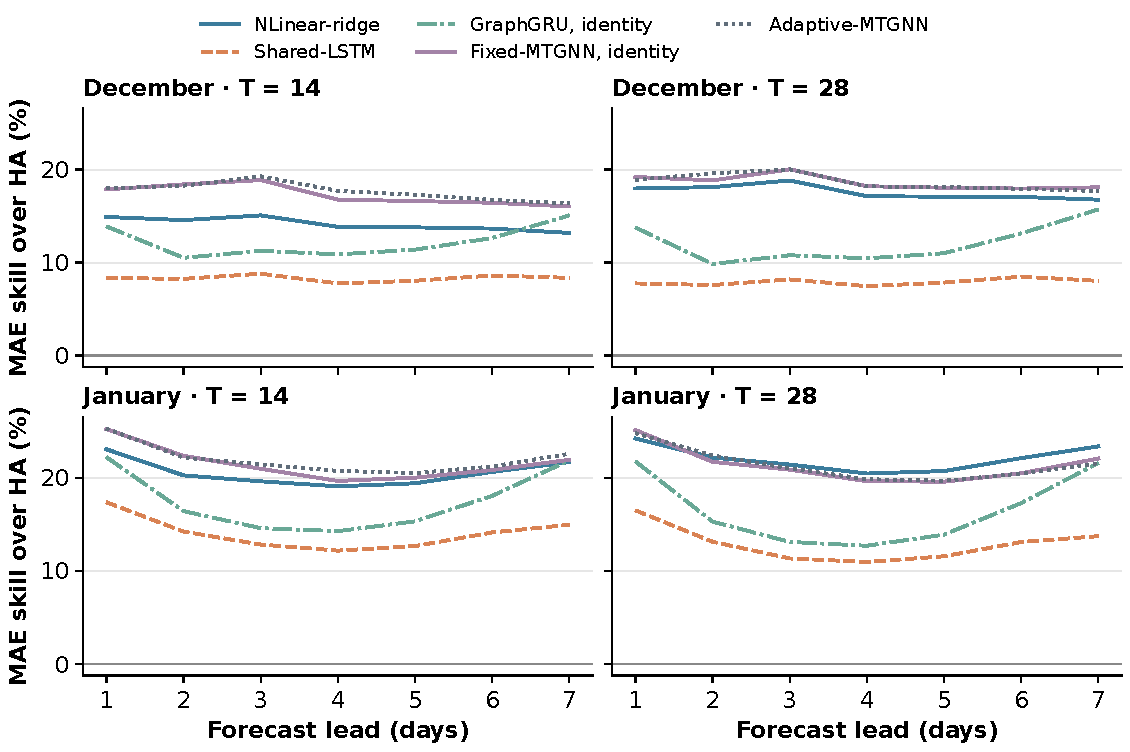
\includegraphics[width=0.96\linewidth]{forecasting_performance_across_horizons.pdf}
\caption{MAE skill relative to HA by forecast lead, computed from five-seed mean errors for neural models. Positive values indicate lower error than HA.}
\label{fig:complete_horizon_skill}
\end{figure}

\begin{table}[!htbp]
\centering
\begingroup
\singlespacing
\fontsize{9pt}{10.5pt}\selectfont
\setlength{\tabcolsep}{4pt}
\renewcommand{\arraystretch}{1.08}
\caption{Paired MAE differences relative to NLinear-ridge. Negative values favor the neural model. Intervals use 2,000 paired resamples and the 2.5th and 97.5th percentiles, conditional on the five fitted seeds. Temporal blocks retain seven consecutive origins and all POIs and leads; the joint sensitivity also resamples occupied 3-km cells.}
\label{tab:forecasting_intervals}
\begin{adjustbox}{max width=\linewidth}
\begin{tabular}{lllrrr}
\toprule
Period & $T$ & Model / adjacency & $\Delta$MAE & Temporal interval & Joint interval \\
\midrule
December & 14 & GraphGRU, identity & +0.028 & [-0.039, +0.082] & [-0.042, +0.093] \\
December & 14 & Fixed-MTGNN, identity & -0.047 & [-0.091, -0.004] & [-0.091, -0.004] \\
December & 14 & Adaptive-MTGNN & -0.052 & [-0.093, -0.014] & [-0.093, -0.014] \\
December & 28 & GraphGRU, identity & +0.081 & [+0.016, +0.132] & [+0.011, +0.146] \\
December & 28 & Fixed-MTGNN, identity & -0.016 & [-0.054, +0.017] & [-0.054, +0.019] \\
December & 28 & Adaptive-MTGNN & -0.016 & [-0.052, +0.014] & [-0.052, +0.016] \\
January & 14 & GraphGRU, identity & +0.048 & [+0.019, +0.069] & [+0.002, +0.092] \\
January & 14 & Fixed-MTGNN, identity & -0.017 & [-0.037, +0.006] & [-0.040, +0.009] \\
January & 14 & Adaptive-MTGNN & -0.023 & [-0.043, -0.002] & [-0.045, +0.001] \\
January & 28 & GraphGRU, identity & +0.088 & [+0.070, +0.109] & [+0.043, +0.132] \\
January & 28 & Fixed-MTGNN, identity & +0.011 & [-0.005, +0.028] & [-0.010, +0.033] \\
January & 28 & Adaptive-MTGNN & +0.011 & [-0.005, +0.027] & [-0.010, +0.032] \\
\bottomrule
\end{tabular}
\end{adjustbox}
\endgroup
\end{table}


\subsubsection{Low-History POIs}
\label{subsubsec:low_history_results}


As discussed in Section~\ref{subsec:data}, POI visit records contain frequent zero observations, and the degree of sparsity varies across locations.
This motivates us to examine how historical visit sparsity affects forecasting performance, particularly whether models can capture occasional positive visits from limited historical information.
We first compare forecasting performance across POI subsets with progressively higher visit densities to assess how model accuracy varies as sparse POIs are excluded.
We then focus on low-history POIs to evaluate positive-demand recovery and false activations on zero-visit events.


\textit{(1) Density Sensitivity.}
We form subsets using overall nonzero frequency, recent-14-day nonzero frequency, and persistence over the training period. Each rule excludes the lowest 10\%, 25\%, 50\%, or 75\% of POIs. GraphGRU with identity adjacency is refitted on each subset at $T=28$ and $H=7$ using the common validation and five-seed protocol.
\begin{table}[!htbp]
\centering
\begingroup
\singlespacing
\fontsize{9pt}{10.5pt}\selectfont
\setlength{\tabcolsep}{4pt}
\renewcommand{\arraystretch}{1.08}
\caption{Visit-density sensitivity at $T=28$, $H=7$. Each subset is selected from training data and refitted at all five seeds. HA uses the identical POIs and forecast events. Nonzero ratios use observed counts within the first 50 calendar days.}
\label{tab:sublevel}
\begin{adjustbox}{max width=\linewidth}
\begin{tabular}{lrrrrr}
\toprule
Subset & POIs & Nonzero ratio & GraphGRU MAE & HA MAE & Skill (\%) \\
\midrule
Full & 9,884 & 0.63 & $1.304\pm 0.008$ & 1.483 & $12.1\pm 0.6$ \\
Dense10 & 8,896 & 0.69 & $1.425\pm 0.006$ & 1.624 & $12.3\pm 0.4$ \\
Dense25 & 7,413 & 0.77 & $1.627\pm 0.005$ & 1.848 & $12.0\pm 0.3$ \\
Dense50 & 4,942 & 0.89 & $2.052\pm 0.008$ & 2.348 & $12.6\pm 0.4$ \\
Dense75 & 2,471 & 0.97 & $2.772\pm 0.032$ & 3.233 & $14.3\pm 1.0$ \\
Recent-dense10 & 8,896 & 0.69 & $1.420\pm 0.005$ & 1.619 & $12.3\pm 0.3$ \\
Recent-dense25 & 7,413 & 0.77 & $1.631\pm 0.005$ & 1.841 & $11.4\pm 0.3$ \\
Recent-dense50 & 4,942 & 0.88 & $2.030\pm 0.008$ & 2.322 & $12.6\pm 0.4$ \\
Recent-dense75 & 2,471 & 0.96 & $2.725\pm 0.018$ & 3.139 & $13.2\pm 0.6$ \\
Persist-dense10 & 8,896 & 0.69 & $1.421\pm 0.005$ & 1.622 & $12.4\pm 0.3$ \\
Persist-dense25 & 7,413 & 0.77 & $1.628\pm 0.004$ & 1.847 & $11.8\pm 0.2$ \\
Persist-dense50 & 4,942 & 0.89 & $2.050\pm 0.008$ & 2.346 & $12.6\pm 0.3$ \\
Persist-dense75 & 2,471 & 0.97 & $2.770\pm 0.031$ & 3.232 & $14.3\pm 1.0$ \\
\bottomrule
\end{tabular}
\end{adjustbox}
\endgroup
\end{table}

Table~\ref{tab:sublevel} compares each refitted model with the historical average on the same retained POIs and forecast events. MAE skill is $100(1-\mathrm{MAE}_{\mathrm{model}}/\mathrm{MAE}_{\mathrm{HA}})$. It is $12.1\%$ on the full panel and ranges from $11.4\%$ to $14.3\%$ across the subsets. The densest overall and persistence subsets attain $14.3\%$ skill, while their larger visit counts raise absolute MAE to approximately $2.77$.

\textit{(2) Zero-Demand Collapse.}
The calendar-based rule identifies 1,944 low-history POIs and 299,376 December test events, of which 53,212 (\(17.8\%\)) have positive visits.
The zero forecast has a low-history MAE of \(0.224\), despite recovering no positive visits.
In Table~\ref{tab:zero_collapse_diagnostic}, Fixed-MTGNN with identity adjacency has lower low-history MAE than GraphGRU, \(0.242\) versus \(0.253\), but also lower DMR, \(7.9\%\) versus \(12.0\%\).
NLinear-ridge and TSB recover more positive visit mass, with DMR of \(23.4\%\) and \(27.5\%\), while activating more zero-visit events.
Thus, the ordering by MAE differs from the ordering by positive-visit recovery.

\begin{table}[!htbp]
\centering
\begingroup
\singlespacing
\fontsize{9pt}{10.5pt}\selectfont
\setlength{\tabcolsep}{4pt}
\renewcommand{\arraystretch}{1.08}
\caption{December forecasting diagnostics at $T=14$, $H=7$. The low-history cohort contains the same 1,944 POIs in every row. DMR, FAR, recall, and AP are percentages; activation uses 0.5 visits.}
\label{tab:zero_collapse_diagnostic}
\begin{adjustbox}{max width=\linewidth}
\begin{tabular}{lrrrrrr}
\toprule
Model / adjacency & All MAE & Low-history MAE & DMR & FAR & Recall & AP \\
\midrule
Zero forecast & 2.411 & 0.224 & 0.0 & 0.0 & 0.0 & 17.8 \\
Historical average & 1.483 & 0.336 & 19.2 & 0.3 & 0.7 & 25.5 \\
NLinear-ridge & 1.273 & 0.301 & 23.4 & 9.2 & 21.0 & 26.8 \\
TSB & 1.337 & 0.334 & 27.5 & 8.9 & 21.9 & 29.2 \\
Shared-LSTM & $1.360\pm 0.013$ & $0.251\pm 0.008$ & $12.0\pm 1.5$ & $1.8\pm 0.2$ & $7.0\pm 0.8$ & $28.0\pm 0.5$ \\
GraphGRU, Identity & $1.302\pm 0.007$ & $0.253\pm 0.007$ & $12.0\pm 1.2$ & $2.2\pm 0.4$ & $7.8\pm 0.9$ & $26.4\pm 0.3$ \\
GraphGRU, NAICS-2 & $1.336\pm 0.007$ & $0.267\pm 0.011$ & $11.7\pm 2.1$ & $4.6\pm 1.1$ & $9.4\pm 2.0$ & $21.6\pm 0.5$ \\
GraphGRU, NAICS-4 & $1.350\pm 0.004$ & $0.261\pm 0.009$ & $11.0\pm 2.1$ & $3.4\pm 0.9$ & $7.9\pm 1.9$ & $21.9\pm 0.5$ \\
Fixed-MTGNN, Identity & $1.227\pm 0.005$ & $0.242\pm 0.011$ & $7.9\pm 1.9$ & $1.0\pm 0.2$ & $4.4\pm 0.8$ & $26.1\pm 0.6$ \\
Fixed-MTGNN, NAICS-2 & $1.222\pm 0.008$ & $0.234\pm 0.008$ & $6.8\pm 1.5$ & $0.9\pm 0.2$ & $4.2\pm 0.7$ & $25.4\pm 0.7$ \\
Fixed-MTGNN, NAICS-4 & $1.222\pm 0.007$ & $0.231\pm 0.006$ & $6.0\pm 1.3$ & $0.8\pm 0.1$ & $3.8\pm 0.5$ & $25.3\pm 1.2$ \\
Adaptive-MTGNN & $1.221\pm 0.007$ & $0.236\pm 0.007$ & $7.4\pm 0.8$ & $1.0\pm 0.1$ & $4.5\pm 0.5$ & $25.9\pm 1.0$ \\
GNN-static & $1.301\pm 0.008$ & $0.245\pm 0.010$ & $10.3\pm 2.3$ & $1.9\pm 0.6$ & $6.9\pm 1.6$ & $25.8\pm 0.9$ \\
\bottomrule
\end{tabular}
\end{adjustbox}
\endgroup
\end{table}


Training loss accounts for a substantial part of this difference.
Table~\ref{tab:calibration_loss} compares the same identity-adjacency architectures under absolute- and squared-error training.
Changing GraphGRU from MAE to MSE raises DMR from \(12.0\%\) to \(23.7\%\), but also raises FAR from \(2.2\%\) to \(7.5\%\) and MAE from \(0.253\) to \(0.328\).
Fixed-MTGNN shows the same shift, with DMR increasing from \(7.9\%\) to \(24.0\%\).
Validation-MAE calibration moves these forecasts toward zero and reduces DMR, showing how minimizing absolute error can favor small forecasts in this cohort.

\begin{table}[!htbp]
\centering
\begingroup
\singlespacing
\fontsize{9pt}{10.5pt}\selectfont
\setlength{\tabcolsep}{4pt}
\renewcommand{\arraystretch}{1.08}
\caption{Loss-function and calibration diagnostics on low-history POIs in December at $T=14$, $H=7$. Neural models use identity adjacency. Calibration minimizes validation MAE. The last two columns use a threshold selected to keep validation FAR at or below 10\%; all rates are percentages.}
\label{tab:calibration_loss}
\begin{adjustbox}{max width=\linewidth}
\begin{tabular}{lrrrrrrr}
\toprule
Model (training loss) & Raw MAE & Raw DMR & Raw FAR & \makecell{Calibrated\\DMR} & \makecell{Calibrated\\FAR} & \makecell{Matched-threshold\\test FAR} & \makecell{Matched-threshold\\test recall} \\
\midrule
GraphGRU (MAE) & $0.253\pm 0.007$ & $12.0\pm 1.2$ & $2.2\pm 0.4$ & $3.0\pm 1.2$ & $0.3\pm 0.1$ & $13.7\pm 0.2$ & $27.9\pm 0.9$ \\
GraphGRU (MSE) & $0.328\pm 0.029$ & $23.7\pm 3.8$ & $7.5\pm 2.3$ & $1.9\pm 0.8$ & $0.2\pm 0.1$ & $13.5\pm 0.2$ & $27.3\pm 0.7$ \\
Fixed-MTGNN (MAE) & $0.242\pm 0.011$ & $7.9\pm 1.9$ & $1.0\pm 0.2$ & $3.5\pm 0.4$ & $0.4\pm 0.0$ & $13.2\pm 0.3$ & $26.0\pm 1.7$ \\
Fixed-MTGNN (MSE) & $0.353\pm 0.025$ & $24.0\pm 3.4$ & $6.6\pm 5.9$ & $2.0\pm 1.2$ & $0.2\pm 0.1$ & $12.6\pm 0.9$ & $24.0\pm 4.1$ \\
Shared-LSTM (MAE) & $0.251\pm 0.008$ & $12.0\pm 1.5$ & $1.8\pm 0.2$ & $6.5\pm 0.2$ & $0.7\pm 0.0$ & $14.4\pm 0.0$ & $30.6\pm 0.1$ \\
Shared-LSTM (MSE) & $0.273\pm 0.011$ & $16.5\pm 2.0$ & $3.0\pm 0.5$ & $6.4\pm 0.2$ & $0.7\pm 0.0$ & $14.3\pm 0.1$ & $30.2\pm 0.1$ \\
NLinear-ridge & 0.301 & 23.4 & 9.2 & 0.1 & 0.0 & 13.0 & 27.0 \\
TSB & 0.334 & 27.5 & 8.9 & 5.8 & 0.7 & 13.5 & 29.2 \\
\bottomrule
\end{tabular}
\end{adjustbox}
\endgroup
\end{table}


\begin{figure}[!htbp]
\centering
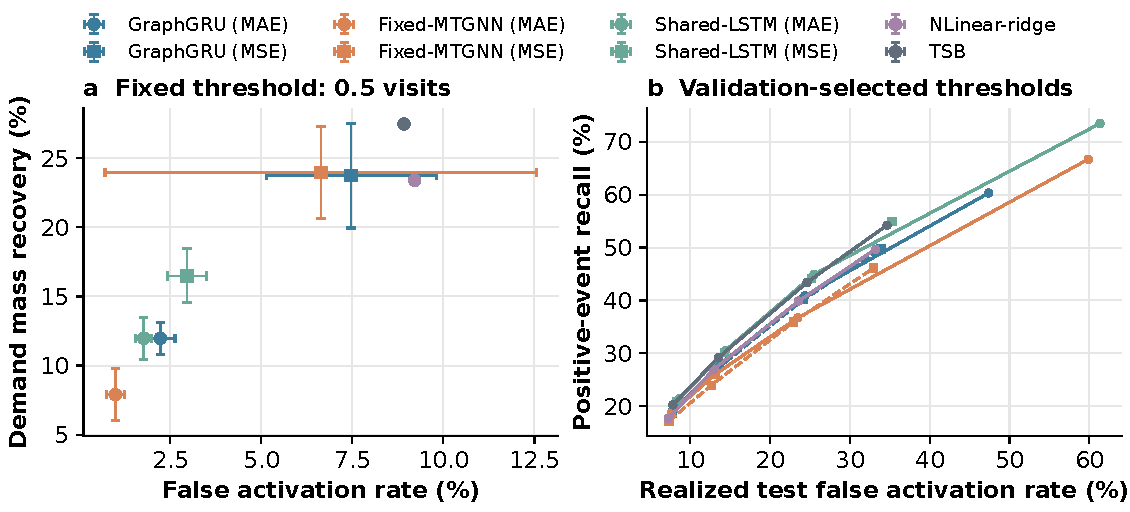
\includegraphics[scale=0.80]{recovery_activation_tradeoff.pdf}
\caption{December diagnostics for the 1,944 low-history POIs at \(T=14\), \(H=7\). Panel (a) shows five-seed means and standard deviations at a fixed 0.5-visit threshold. Panel (b) reports test recall and realized test FAR at thresholds selected for validation FAR targets of \(5\%,10\%,20\%,30\%\).}
\label{fig:recovery_activation_tradeoff}
\end{figure}

Threshold matching gives a different comparison from forecast magnitude alone.
At the \(10\%\) validation-FAR target, GraphGRU trained with MAE attains \(27.9\%\) December recall, compared with \(30.6\%\) for Shared-LSTM and \(29.2\%\) for TSB; their realized test FARs are \(13.7\%\), \(14.4\%\), and \(13.5\%\), respectively.
GraphGRU trained with MSE has similar matched-threshold recall of \(27.3\%\), despite its much larger raw DMR.
Figure~\ref{fig:recovery_activation_tradeoff} shows this distinction across the four validation targets.
With the same fitted models and thresholds in January, recall is \(39.3\%\) for MAE-trained GraphGRU, \(42.7\%\) for Shared-LSTM, and \(41.2\%\) for TSB, at realized FARs of \(14.6\%\), \(15.8\%\), and \(14.7\%\).
Forecast magnitude and matched-threshold detection describe different aspects of intermittent-visit recovery; Shared-LSTM and TSB achieve higher matched-threshold recall than GraphGRU in these comparisons.

\begin{table}[!htbp]
\centering
\begingroup
\singlespacing
\fontsize{9pt}{10.5pt}\selectfont
\setlength{\tabcolsep}{4pt}
\renewcommand{\arraystretch}{1.08}
\caption{January diagnostics for the fixed low-history cohort at $T=14$, $H=7$. Models, calibration, and activation thresholds retain their original validation choices. All rates are percentages.}
\label{tab:january_low_history}
\begin{adjustbox}{max width=\linewidth}
\begin{tabular}{lrrrrrr}
\toprule
Model (training loss) & MAE & DMR & FAR & AP & Matched test FAR & Matched test recall \\
\midrule
GraphGRU (MAE) & $0.331\pm 0.006$ & $27.7\pm 0.9$ & $3.2\pm 0.4$ & $41.6\pm 0.3$ & $14.6\pm 0.3$ & $39.3\pm 0.9$ \\
GraphGRU (MSE) & $0.395\pm 0.026$ & $38.0\pm 2.8$ & $8.5\pm 2.3$ & $42.9\pm 0.5$ & $14.3\pm 0.3$ & $38.7\pm 0.8$ \\
Fixed-MTGNN (MAE) & $0.323\pm 0.010$ & $23.4\pm 1.5$ & $1.7\pm 0.3$ & $42.1\pm 0.7$ & $14.1\pm 0.4$ & $38.1\pm 1.6$ \\
Fixed-MTGNN (MSE) & $0.422\pm 0.021$ & $35.9\pm 2.8$ & $7.7\pm 5.8$ & $41.9\pm 1.3$ & $13.4\pm 1.0$ & $35.0\pm 4.4$ \\
Shared-LSTM (MAE) & $0.332\pm 0.006$ & $26.9\pm 1.3$ & $2.8\pm 0.3$ & $43.3\pm 0.7$ & $15.8\pm 0.1$ & $42.7\pm 0.1$ \\
Shared-LSTM (MSE) & $0.349\pm 0.010$ & $31.5\pm 1.6$ & $4.2\pm 0.6$ & $44.3\pm 0.3$ & $15.5\pm 0.1$ & $42.2\pm 0.1$ \\
NLinear-ridge & 0.368 & 39.4 & 9.7 & 42.5 & 13.3 & 37.9 \\
TSB & 0.402 & 41.3 & 10.2 & 45.0 & 14.7 & 41.2 \\
\bottomrule
\end{tabular}
\end{adjustbox}
\endgroup
\end{table}



\subsection{Information Sharing among POIs}
\label{subsec:information_sharing_results}


The low-history evaluation shows that information from related POIs affects both positive-demand recovery and false activation.
We further investigate these effects at the individual prediction level and examine how different groups of neighboring POIs contribute to forecast changes.
The analysis combines graph-transfer regime comparisons with neighbor-group perturbations.


\subsubsection{Alternative Adjacency Matrices}
\label{subsubsec:adjacency_results}

We compare functional and identity adjacency on the same 1,935 low-history POIs with at least one NAICS-4 peer, using \(T=14\) and \(H=7\).
The December and January evaluations contain 297,990 and 338,625 scored events, respectively.
Target and neighbor evidence are classified using validation-period medians, before observing the test outcomes.
Table~\ref{tab:graph_transfer_summary} reports MAE gain within these evidence strata. Figure~\ref{fig:counterfactual_graph_transfer_map} resolves the pattern using validation-defined sextile cutpoints, with duplicate boundaries merged.

\begin{table}[!htbp]
\centering
\begingroup
\singlespacing
\fontsize{9pt}{10.5pt}\selectfont
\setlength{\tabcolsep}{4pt}
\renewcommand{\arraystretch}{1.08}
\caption{MAE gain over identity adjacency within validation-defined target/neighbor evidence strata at $T=14$, $H=7$. Values are means and standard deviations across five fitted seeds; positive values indicate lower error under functional adjacency.}
\label{tab:graph_transfer_summary}
\begin{adjustbox}{max width=\linewidth}
\begin{tabular}{lrrrr}
\toprule
Target / neighbor evidence & Dec. NAICS-2 & Dec. NAICS-4 & Jan. NAICS-2 & Jan. NAICS-4 \\
\midrule
Low / low & $-0.005\pm 0.004$ & $0.002\pm 0.006$ & $-0.012\pm 0.005$ & $0.001\pm 0.006$ \\
Low / high & $-0.056\pm 0.012$ & $-0.037\pm 0.007$ & $-0.191\pm 0.025$ & $-0.043\pm 0.007$ \\
High / low & $0.015\pm 0.009$ & $0.027\pm 0.014$ & $0.005\pm 0.007$ & $0.020\pm 0.011$ \\
High / high & $-0.032\pm 0.011$ & $-0.020\pm 0.010$ & $-0.118\pm 0.017$ & $-0.025\pm 0.009$ \\
\bottomrule
\end{tabular}
\end{adjustbox}
\endgroup
\end{table}


\begin{figure}[!htbp]
\centering
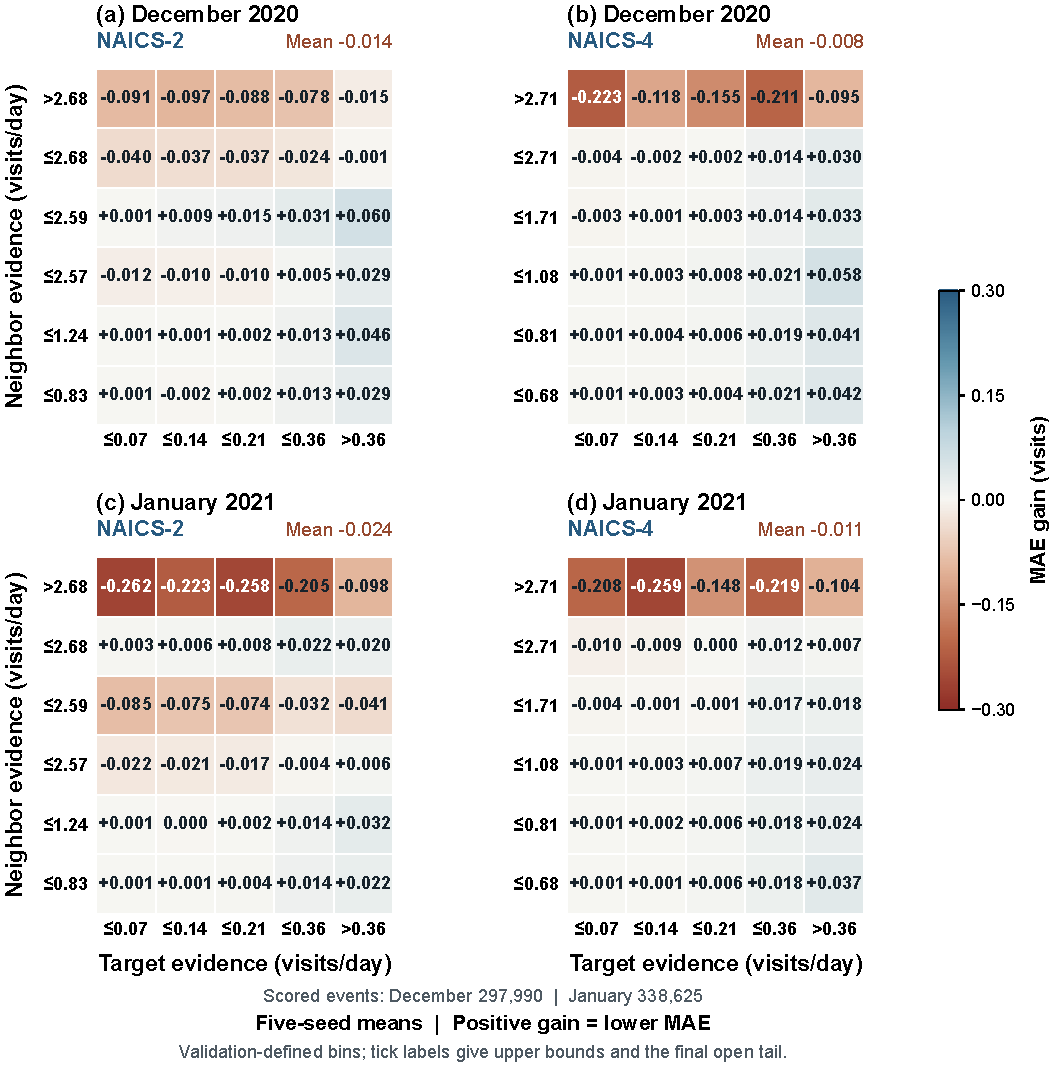
\includegraphics[width=\linewidth]{art/pre_outcome_graph_transfer.pdf}
\caption{Five-seed mean MAE gain over identity adjacency across target and neighbor evidence at \(T=14\), \(H=7\). Validation sextile cutpoints define the bins; ticks show successive upper bounds and the open tail. Positive gains indicate lower error under functional adjacency. Panel means weight cells by scored events; each cell contains at least 602 events. Fitted models and bin boundaries remain fixed in January.}
\label{fig:counterfactual_graph_transfer_map}
\end{figure}

Neighbor utility varies with both target evidence and neighbor activity.
For low target evidence and high neighbor evidence, NAICS-2 increases MAE by \(0.056\) visits in December and \(0.191\) in January; the corresponding increases under NAICS-4 are \(0.037\) and \(0.043\).
When target evidence is high and neighbor evidence is low, both graphs instead yield positive mean gains in both months.
Across all matched targets, NAICS-2 increases MAE by \(0.014\) in December, with a paired joint temporal--spatial 95\% interval of \([0.006,0.022]\), and by \(0.024\) in January, with an interval of \([0.013,0.037]\).
The corresponding NAICS-4 increases are \(0.008\) and \(0.011\); its December interval \([-0.001,0.017]\) includes zero.
These comparisons locate the largest errors in an evidence stratum that can be identified before the target visits are realized.

NAICS-4 and top category induce the same partition of the 9,884 POIs into 134 groups and therefore represent one graph specification.
NAICS-2 forms 22 groups, with a mean non-self degree of 1,586.5 compared with 767.0 under NAICS-4.
The clique comparison consequently changes both functional detail and neighborhood size.

Table~\ref{tab:semantic_granularity_transfer} holds the non-self degree fixed within each target. At $k=10$, NAICS-4 reduces December MAE relative to random neighbors by $0.0082$ for GraphGRU and $0.0056$ for Fixed-MTGNN, with joint temporal and 3-km spatial intervals of $[-0.0140,-0.0020]$ and $[-0.0069,-0.0044]$. The corresponding January reductions are $0.0126$ and $0.0037$. Relative to identity adjacency, however, GraphGRU error increases by $0.0645$ in December, while Fixed-MTGNN error decreases by $0.0080$. Functional similarity thus helps identify neighbors within a fixed-size graph, while the utility of graph propagation depends on the forecasting architecture.

\begin{table}[!htbp]
\centering
\begingroup
\singlespacing
\fontsize{9pt}{10.5pt}\selectfont
\setlength{\tabcolsep}{4pt}
\renewcommand{\arraystretch}{1.08}
\caption{Degree-controlled graph comparison at $T=14$, $H=7$. Each target has the same non-self degree under NAICS-2, NAICS-4, and random graphs, capped by $k$ and its available NAICS-4 peers. Values are five-seed MAE means and standard deviations.}
\label{tab:semantic_granularity_transfer}
\begin{adjustbox}{max width=\linewidth}
\begin{tabular}{llrrrrrr}
\toprule
Model & $k$ & Dec. NAICS-2 & Dec. NAICS-4 & Dec. random & Jan. NAICS-2 & Jan. NAICS-4 & Jan. random \\
\midrule
GraphGRU & 5 & $1.394\pm 0.002$ & $1.395\pm 0.012$ & $1.397\pm 0.001$ & $1.405\pm 0.001$ & $1.401\pm 0.012$ & $1.409\pm 0.003$ \\
GraphGRU & 10 & $1.375\pm 0.004$ & $1.366\pm 0.004$ & $1.374\pm 0.007$ & $1.387\pm 0.003$ & $1.375\pm 0.001$ & $1.388\pm 0.006$ \\
GraphGRU & 20 & $1.362\pm 0.006$ & $1.360\pm 0.006$ & $1.359\pm 0.010$ & $1.376\pm 0.008$ & $1.369\pm 0.007$ & $1.375\pm 0.011$ \\
\addlinespace[3pt]
Fixed-MTGNN & 5 & $1.226\pm 0.005$ & $1.223\pm 0.003$ & $1.226\pm 0.005$ & $1.250\pm 0.008$ & $1.246\pm 0.004$ & $1.247\pm 0.004$ \\
Fixed-MTGNN & 10 & $1.220\pm 0.005$ & $1.219\pm 0.005$ & $1.224\pm 0.006$ & $1.242\pm 0.007$ & $1.240\pm 0.008$ & $1.244\pm 0.007$ \\
Fixed-MTGNN & 20 & $1.224\pm 0.006$ & $1.221\pm 0.005$ & $1.224\pm 0.006$ & $1.247\pm 0.007$ & $1.242\pm 0.010$ & $1.247\pm 0.009$ \\
\bottomrule
\end{tabular}
\end{adjustbox}
\endgroup
\end{table}


The spatial and visit-correlation alternatives in Table~\ref{tab:spatial_graphs} show the same architectural distinction. All three GraphGRU alternatives have higher MAE than identity adjacency in both periods. Distance-neighbor propagation reduces Fixed-MTGNN MAE by $0.0051$ in December and $0.0045$ in January, with joint intervals of $[-0.0089,-0.0022]$ and $[-0.0071,-0.0020]$.

\begin{table}[!htbp]
\centering
\begingroup
\singlespacing
\fontsize{9pt}{10.5pt}\selectfont
\setlength{\tabcolsep}{4pt}
\renewcommand{\arraystretch}{1.08}
\caption{Additional fixed spatial and visit-correlation graphs at $T=14$, $H=7$. Values are five-seed MAE means and standard deviations.}
\label{tab:spatial_graphs}
\begin{adjustbox}{max width=\linewidth}
\begin{tabular}{llrr}
\toprule
Model & Adjacency & December & January \\
\midrule
GraphGRU & Distance KNN & $1.375\pm 0.010$ & $1.381\pm 0.009$ \\
GraphGRU & Distance RBF & $1.348\pm 0.011$ & $1.357\pm 0.010$ \\
GraphGRU & Visit correlation & $1.346\pm 0.010$ & $1.358\pm 0.011$ \\
Fixed-MTGNN & Distance KNN & $1.222\pm 0.008$ & $1.242\pm 0.009$ \\
\bottomrule
\end{tabular}
\end{adjustbox}
\endgroup
\end{table}


The outcome-conditioned transfer regimes remain descriptive assignments; in particular, negative MAE gain for a zero-visit event with positive graph lift follows directly from its definition.


\subsubsection{Related-POI Perturbation}
\label{subsubsec:perturbation_results}

We perturb matched neighbor sets while holding each fitted GraphGRU and its adjacency fixed.
Each target receives the same intervention size across selection rules and graphs, between one and ten neighbors, with a mean of 9.88.
Table~\ref{tab:metric_targeted_perturbation_naics4} reports the NAICS-4 results over all matched target events.
The disconnected-node control gives zero forecast change in every graph, seed, and evaluation month.

\begin{table}[!htbp]
\centering
\begingroup
\singlespacing
\fontsize{9pt}{10.5pt}\selectfont
\setlength{\tabcolsep}{4pt}
\renewcommand{\arraystretch}{1.08}
\caption{Matched neighbor interventions under NAICS-4 at $T=14$, $H=7$, averaged over five seeds. Every rule intervenes on the same number of neighbors for each target. Removed false activations and lost positive activations are percentages of their originally activated zero-visit and positive-visit events, respectively.}
\label{tab:metric_targeted_perturbation_naics4}
\begin{adjustbox}{max width=\linewidth}
\begin{tabular}{llrrrr}
\toprule
Period & Neighbor group & \makecell{Reduction\\per neighbor} & $\Delta\mathrm{MAE}$ & \makecell{False activations\\removed (\%)} & \makecell{Positive activations\\lost (\%)} \\
\midrule
December & Training-active & $0.0026\pm 0.0003$ & $-0.016\pm 0.002$ & $40.1\pm 7.8$ & $22.5\pm 4.0$ \\
 & Recent-active & $0.0025\pm 0.0003$ & $-0.016\pm 0.002$ & $39.7\pm 7.8$ & $22.1\pm 4.2$ \\
 & Correlated & $0.0013\pm 0.0001$ & $-0.006\pm 0.001$ & $17.8\pm 3.5$ & $9.4\pm 1.4$ \\
 & Random & $0.0013\pm 0.0001$ & $-0.006\pm 0.001$ & $17.9\pm 3.5$ & $8.9\pm 1.1$ \\
 & Matched replacement & $0.0006\pm 0.0001$ & $-0.003\pm 0.001$ & $17.1\pm 2.0$ & $9.5\pm 0.8$ \\
\addlinespace[3pt]
January & Training-active & $0.0030\pm 0.0003$ & $-0.016\pm 0.001$ & $32.5\pm 5.6$ & $10.7\pm 1.1$ \\
 & Recent-active & $0.0029\pm 0.0003$ & $-0.016\pm 0.002$ & $32.3\pm 5.7$ & $10.5\pm 1.1$ \\
 & Correlated & $0.0014\pm 0.0001$ & $-0.005\pm 0.001$ & $15.2\pm 2.5$ & $4.7\pm 0.6$ \\
 & Random & $0.0014\pm 0.0001$ & $-0.006\pm 0.000$ & $14.9\pm 2.3$ & $4.4\pm 0.5$ \\
 & Matched replacement & $0.0008\pm 0.0001$ & $-0.004\pm 0.000$ & $16.3\pm 1.6$ & $5.5\pm 0.2$ \\
\bottomrule
\end{tabular}
\end{adjustbox}
\endgroup
\end{table}


Zeroing neighbors with the highest training activity reduces December MAE by \(0.016\) visits, compared with \(0.006\) for random neighbors of the same size.
Its paired joint temporal--spatial 95\% interval is \([-0.023,-0.010]\) visits.
Recent-active neighbors produce a similar reduction, while correlation-based selection is close to random selection.
The ordering persists in January, when the MAE reductions are \(0.016\) for training-active neighbors and \(0.006\) for random neighbors.
Replacing active-neighbor histories with activity-matched external histories produces smaller reductions of \(0.003\) and \(0.004\) visits in the two months.
Thus, the effect of setting histories to zero partly reflects the amount of activity removed; it exceeds the effect of replacing histories with comparable training activity.

\begin{figure}[!htbp]
\centering
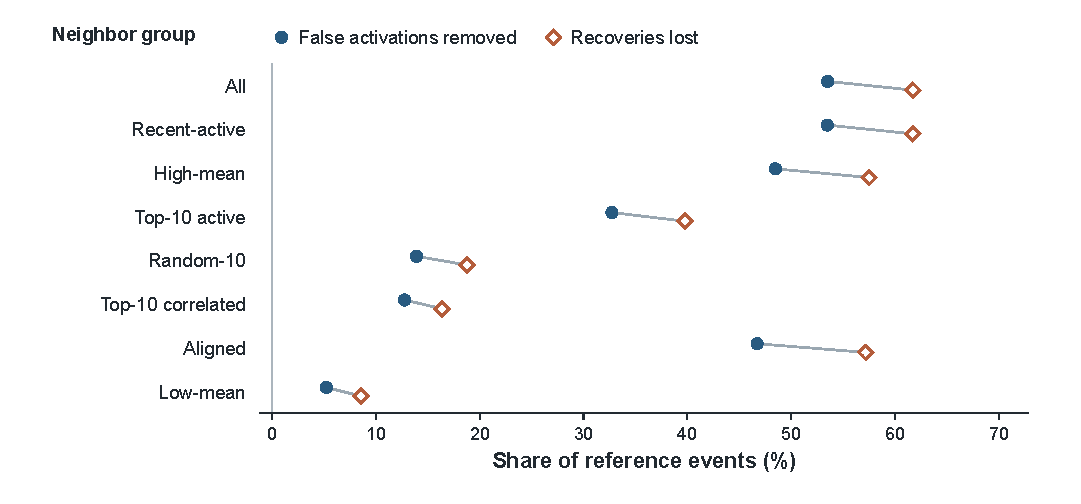
\includegraphics[scale=0.80]{art/neighbor_perturbation_tradeoff.pdf}
\caption{Matched neighbor interventions under NAICS-4 at \(T=14\), \(H=7\). Points and bars show five-seed means and standard deviations. Each percentage uses its own originally activated zero-visit or positive-visit events as the denominator.}
\label{fig:neighbor_perturbation_tradeoff}
\end{figure}

The reduction in aggregate error comes with lost positive-event detections.
In December, zeroing training-active neighbors removes \(40.1\%\) of original false activations and \(22.5\%\) of original positive activations; in January, the corresponding fractions are \(32.5\%\) and \(10.7\%\).
Recent-active selection has nearly the same tradeoff, as Figure~\ref{fig:neighbor_perturbation_tradeoff} shows.
The activity-matched replacement removes \(17.1\%\) of false activations and \(9.5\%\) of positive activations in December.
Active neighbors therefore support both correct detections and false activations, and lower aggregate MAE after their removal does not imply better detection of intermittent visits.


\subsubsection{Spatial Activity Prioritization}
\label{subsubsec:activity_prioritization}
We also rank the 256 occupied 1-km cells by predicted visits and measure the observed visit mass captured by fixed budgets of 13, 26, and 52 cells. Table~\ref{tab:activity_coverage} reports coverage for each model, averaging per-seed selections over origins and leads.
At the 26-cell budget, HA captures $48.01\%$ of December visits, compared with $48.22\%$ for Fixed-MTGNN with identity adjacency and $48.29\%$ for NLinear-ridge. The corresponding gains are $0.20$ percentage points (paired 95\% interval $[0.16,0.25]$) and $0.28$ points ($[0.24,0.32]$). January gains are $0.15$ points ($[0.01,0.26]$) and $0.23$ points ($[0.09,0.34]$). Historical spatial concentration accounts for most captured visits, with modest gains from the fitted forecasts. This outcome measures observed-visit coverage under a fixed inspection budget.

\begin{table}[!htbp]
\centering
\begingroup
\singlespacing
\fontsize{9pt}{10.5pt}\selectfont
\setlength{\tabcolsep}{4pt}
\renewcommand{\arraystretch}{1.08}
\caption{Observed-visit coverage (\%) when prioritizing 13, 26, or 52 of the 256 occupied 1-km cells at $T=14$, $H=7$. Selection ranks each fitted model separately; reported values average coverage across seeds, origins, and leads. The last row ranks cells retrospectively by observed visits. Paired gains use unrounded coverage values.}
\label{tab:activity_coverage}
\begin{adjustbox}{max width=\linewidth}
\begin{tabular}{lrrrrrr}
\toprule
Model & Dec., 13 & Dec., 26 & Dec., 52 & Jan., 13 & Jan., 26 & Jan., 52 \\
\midrule
Historical average & 33.95 & 48.01 & 65.78 & 34.33 & 48.31 & 66.28 \\
Weekday historical average & 34.25 & 48.32 & 66.01 & 34.43 & 48.71 & 66.60 \\
Seasonal naive & 34.20 & 48.24 & 65.96 & 34.32 & 48.40 & 66.27 \\
NLinear-ridge & 34.26 & 48.29 & 66.07 & 34.37 & 48.54 & 66.44 \\
TSB & 34.05 & 48.08 & 65.93 & 34.25 & 48.37 & 66.31 \\
Shared-LSTM & $33.94\pm 0.00$ & $47.84\pm 0.01$ & $65.90\pm 0.01$ & $34.25\pm 0.05$ & $48.08\pm 0.04$ & $66.24\pm 0.02$ \\
GraphGRU, identity & $33.85\pm 0.01$ & $47.95\pm 0.02$ & $65.93\pm 0.02$ & $33.99\pm 0.01$ & $48.17\pm 0.03$ & $66.22\pm 0.02$ \\
Fixed-MTGNN, identity & $34.13\pm 0.05$ & $48.22\pm 0.03$ & $66.06\pm 0.00$ & $34.24\pm 0.02$ & $48.45\pm 0.04$ & $66.38\pm 0.02$ \\
Adaptive-MTGNN & $34.14\pm 0.03$ & $48.24\pm 0.03$ & $66.07\pm 0.01$ & $34.25\pm 0.01$ & $48.48\pm 0.02$ & $66.39\pm 0.02$ \\
GNN-static & $33.87\pm 0.03$ & $47.93\pm 0.06$ & $65.94\pm 0.01$ & $34.02\pm 0.05$ & $48.15\pm 0.06$ & $66.21\pm 0.03$ \\
\addlinespace[3pt]
Observed-ranking upper bound & 34.48 & 48.85 & 66.70 & 34.57 & 48.96 & 66.95 \\
\bottomrule
\end{tabular}
\end{adjustbox}
\endgroup
\end{table}


\subsection{Explaining POI Visit Predictions}
\label{subsec:explanation_results}


Following the analysis of cross-POI information transfer, we examine the contributions of the history and static attributes of a POI using the five GNN-static fits with identity adjacency at \(T=14\), \(H=7\).
With numeric inputs standardized, history accounts for \(57.7\%\) of the mean Gradient \(\times\) Input share among eligible POIs, compared with \(22.5\%\) for identity, \(18.3\%\) for parent, \(1.0\%\) for other attributes, and \(0.45\%\) for location.
These are normalized attribution magnitudes; the subsequent retraining experiments assess whether each input improves predictive accuracy.

\subsubsection{POI Attribution Regimes}
\label{subsubsec:attribution_regimes}
Attribution methods assign substantially different shares to the same feature groups.
Figure~\ref{fig:attribution_method_comparison} compares the methods on the common eligible POIs in the fixed sample of 1,024 locations.
In December, the mean history share is \(58.1\%\) under Gradient \(\times\) Input and \(74.6\%\) and \(87.2\%\) under the two IG references.
The parent share falls from \(18.2\%\) to \(2.1\%\) and \(1.1\%\), respectively.
January reproduces this pattern, so attribution magnitudes depend strongly on the method and reference input even with the fitted predictor held fixed.

\begin{figure}[!htbp]
\centering
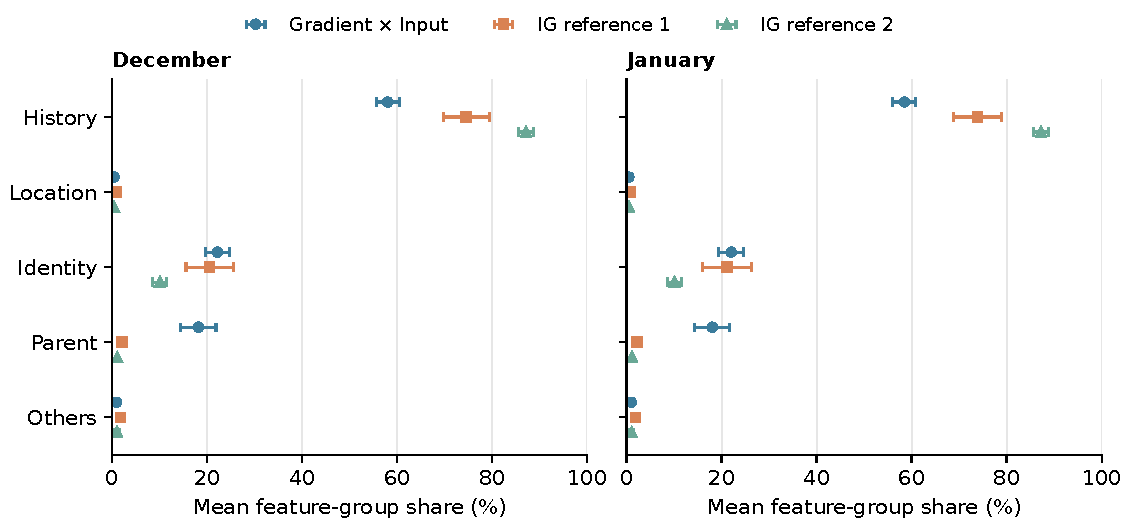
\includegraphics[scale=0.65]{art/attribution_method_comparison.pdf}
\caption{Mean feature-group shares on the common eligible POIs in the 1,024-POI sample at \(T=14\), \(H=7\). Points and bars show means and standard deviations across the five fitted seeds. Each method uses the same eight origins and seven leads within a month.}
\label{fig:attribution_method_comparison}
\end{figure}

The resulting regime assignments also vary across fitted seeds and attribution methods, as Table~\ref{tab:attribution_stability} shows.
December agreement between Gradient \(\times\) Input and the two IG references is only \(21.3\%\) and \(22.9\%\), and mean agreement across the ten fitted-seed pairs is \(50.4\%\).
January gives similar method agreement of \(21.2\%\) and \(23.1\%\).
Holding the fitted models fixed, the December and January consensus assignments agree for \(74.2\%\) of the 9,817 POIs assigned in both months.
Thus, changing the attribution method alters regime membership more than moving these fitted models to the following month.
The category patterns and map in Appendix~\ref{app:descriptive_attribution} describe the Gradient \(\times\) Input representation.
All 1,895 POIs assigned to the parent-driven consensus regime lack a recorded parent place, so their attribution concerns the learned missing-parent category.
We therefore examine recorded parent places separately in Section~\ref{subsubsec:parent_results} and assess feature utility through retraining.

\begin{table}[!htbp]
\centering
\begingroup
\singlespacing
\fontsize{9pt}{10.5pt}\selectfont
\setlength{\tabcolsep}{4pt}
\renewcommand{\arraystretch}{1.08}
\caption{Attribution stability. Method comparisons use the same 1,024 sampled POIs and forecast events; regime agreement reports the mean and SD across five seeds. The last row in each period averages the ten seed-pair comparisons over all eligible POIs. Remaining columns are mean Spearman rank correlations for feature-group shares. Zero-attribution profiles are excluded.}
\label{tab:attribution_stability}
\begin{adjustbox}{max width=\linewidth}
\begin{tabular}{llrrrrrr}
\toprule
Period & Comparison & Agreement (\%) & History & Location & Identity & Parent & Others \\
\midrule
December & Gradient $\times$ Input / IG 1 & $21.3\pm 7.7$ & -0.06 & 0.51 & -0.07 & -0.30 & 0.05 \\
December & Gradient $\times$ Input / IG 2 & $22.9\pm 7.1$ & -0.12 & 0.90 & -0.20 & -0.30 & 0.06 \\
December & IG 1 / IG 2 & $24.8\pm 2.8$ & 0.08 & 0.61 & 0.03 & 1.00 & -0.77 \\
December & Different fitted seeds & 50.4 & 0.77 & 0.86 & 0.69 & 0.63 & 0.59 \\
January & Gradient $\times$ Input / IG 1 & $21.2\pm 8.8$ & -0.04 & 0.53 & -0.06 & -0.30 & 0.04 \\
January & Gradient $\times$ Input / IG 2 & $23.1\pm 7.3$ & -0.16 & 0.90 & -0.25 & -0.29 & 0.07 \\
January & IG 1 / IG 2 & $25.0\pm 3.2$ & 0.09 & 0.63 & 0.03 & 1.00 & -0.78 \\
January & Different fitted seeds & 50.2 & 0.77 & 0.86 & 0.68 & 0.61 & 0.60 \\
\bottomrule
\end{tabular}
\end{adjustbox}
\endgroup
\end{table}



\subsubsection{Parent-Place Information}
\label{subsubsec:parent_results}

POIs located within larger destinations, such as shopping malls and medical facilities, may share contextual characteristics with their parent places.
We further examine how parent-place information contributes to forecasts for these embedded POIs relative to their own historical visits and other static attributes.
The analysis covers 581 POIs with 233 recorded parent places. Frequency pooling retains two parent labels separately and combines the remaining 231, so the attribution primarily describes this coarse parent-place encoding. We compare its attribution across embedded POI groups.


\begin{table}[!htbp]
\centering
\begingroup
\singlespacing
\fontsize{9pt}{10.5pt}\selectfont
\setlength{\tabcolsep}{4pt}
\renewcommand{\arraystretch}{1.08}
\caption{December attribution and feature-removal effects on POIs with a recorded parent. Shares exclude zero-attribution profiles; errors use all POIs in each group. The last column is removed-feature MAE minus full-model MAE. Entries report five-seed means and standard deviations.}
\label{tab_parent}
\begin{adjustbox}{max width=\linewidth}
\begin{tabular}{lrrrr}
\toprule
Embedded POI group & POIs & Parent share (\%) & Full MAE & $\Delta\mathrm{MAE}$ \\
\midrule
All embedded POIs & 581 & $12.0\pm 2.5$ & $1.454\pm 0.009$ & $-0.002\pm 0.006$ \\
Schools, campuses, and education-related POIs & 8 & $11.5\pm 3.2$ & $1.616\pm 0.024$ & $-0.009\pm 0.013$ \\
Repair, towing, and irregular services & 5 & $9.4\pm 2.6$ & $0.463\pm 0.010$ & $-0.002\pm 0.005$ \\
Restaurants and cafes & 170 & $11.6\pm 2.0$ & $1.519\pm 0.006$ & $-0.004\pm 0.005$ \\
Shopping centers and office-building POIs & 112 & $12.7\pm 3.3$ & $1.323\pm 0.011$ & $-0.000\pm 0.004$ \\
Clinics and medical services & 111 & $13.1\pm 3.1$ & $1.837\pm 0.026$ & $-0.000\pm 0.021$ \\
Pharmacies and health-related retail & 18 & $10.8\pm 2.1$ & $1.809\pm 0.009$ & $-0.016\pm 0.005$ \\
Small local businesses & 104 & $11.2\pm 2.1$ & $1.177\pm 0.006$ & $-0.003\pm 0.004$ \\
Bars and nightlife POIs & 12 & $9.6\pm 1.7$ & $0.841\pm 0.003$ & $0.005\pm 0.004$ \\
Grocery and daily retail & 41 & $12.1\pm 2.7$ & $1.319\pm 0.003$ & $-0.001\pm 0.004$ \\
\bottomrule
\end{tabular}
\end{adjustbox}
\endgroup
\end{table}


Table~\ref{tab_parent} shows a mean parent attribution share of \(12.0\%\) across eligible embedded POIs in December, with a five-seed standard deviation of 2.5 percentage points.
The corresponding January share is \(11.8\%\).
December shares range from \(9.4\%\) for repair services to \(13.1\%\) for clinics, while clinic forecasts have a higher MAE than the other displayed groups.
The feature-removal comparison in Table~\ref{tab:parent_ablation} gives December MAE $1.454$ for the full model and $1.451$ after removing parent information from the harmonized metadata. The paired difference, defined as removed-feature MAE minus full-model MAE, is $-0.0023$, with a 95\% joint temporal and 1-km spatial interval of $[-0.0068,0.0014]$. January MAE changes from $1.469$ to $1.467$. With earlier metadata, the corresponding full and removed-feature values are $1.436$ and $1.436$ in December, and $1.453$ and $1.452$ in January. Parent-feature removal therefore has a small average effect in both metadata settings.

\begin{table}[!htbp]
\centering
\begingroup
\singlespacing
\fontsize{9pt}{10.5pt}\selectfont
\setlength{\tabcolsep}{4pt}
\renewcommand{\arraystretch}{1.08}
\caption{Parent-feature removal on the same 581 POIs with a recorded parent in the harmonized metadata. Earlier metadata uses the earliest available 2020 record and its parent-identifier crosswalk; POI membership is held fixed for comparison. Paired differences use unrounded seed-level errors.}
\label{tab:parent_ablation}
\begin{adjustbox}{max width=\linewidth}
\begin{tabular}{llrr}
\toprule
Period & Metadata & Full MAE & Without-parent MAE \\
\midrule
December & Harmonized metadata & $1.454\pm 0.009$ & $1.451\pm 0.005$ \\
December & Earlier metadata & $1.436\pm 0.021$ & $1.436\pm 0.024$ \\
January & Harmonized metadata & $1.469\pm 0.010$ & $1.467\pm 0.008$ \\
January & Earlier metadata & $1.453\pm 0.019$ & $1.452\pm 0.025$ \\
\bottomrule
\end{tabular}
\end{adjustbox}
\endgroup
\end{table}


Across recorded-parent POIs, the mean within-seed Spearman correlation between parent attribution share and the MAE increase after removal is $-0.048$ in December and $-0.072$ in January. These weak associations describe limited correspondence between attribution magnitude and predictive benefit.

\subsubsection{Category and Industry Granularity}
\label{subsubsec:granularity_results}

Finally, we examine how category labels and industry codes at different levels of granularity contribute to POI visit predictions, identifying which semantic descriptors have the largest attribution.
Top category, sub-category, NAICS-2, and NAICS-4 are encoded jointly in GNN-static, with the attribution share of each descriptor measured relative to all input components.
We aggregate absolute attribution over the sampled origins and leads for each POI and identify the descriptor with the largest semantic attribution, excluding POIs with zero semantic attribution.
Table~\ref{tab:semantic_granularity} reports the five-seed means and standard deviations of these shares and dominance frequencies in both evaluation periods.

\begin{table}[!htbp]
\centering
\begingroup
\singlespacing
\fontsize{9pt}{10.5pt}\selectfont
\setlength{\tabcolsep}{4pt}
\renewcommand{\arraystretch}{1.08}
\caption{Semantic attribution under jointly encoded descriptors. Mean share (\%) uses total attribution across all inputs. Dominance (\%) is the fraction of POIs for which that descriptor has the largest aggregated semantic attribution; POIs with zero semantic attribution are excluded. Values are five-seed means and SDs.}
\label{tab:semantic_granularity}
\begin{adjustbox}{max width=\linewidth}
\begin{tabular}{lrrrr}
\toprule
Descriptor & Dec. share & Dec. dominance & Jan. share & Jan. dominance \\
\midrule
Top category & $1.4\pm 0.4$ & $10.6\pm 6.6$ & $1.4\pm 0.4$ & $10.7\pm 6.7$ \\
Sub-category & $1.2\pm 0.6$ & $4.9\pm 2.5$ & $1.2\pm 0.6$ & $4.9\pm 2.6$ \\
NAICS-2 & $2.9\pm 0.9$ & $67.2\pm 11.2$ & $2.9\pm 0.9$ & $67.6\pm 11.0$ \\
NAICS-4 & $1.7\pm 0.6$ & $17.3\pm 11.2$ & $1.7\pm 0.6$ & $16.9\pm 11.1$ \\
\bottomrule
\end{tabular}
\end{adjustbox}
\endgroup
\end{table}


NAICS-2 has the largest mean share among the four descriptors, at \(2.9\%\) of total attribution, and is dominant for \(67.2\%\) of eligible POIs in December and \(67.6\%\) in January.
Its dominance frequency varies across fitted seeds, with standard deviations of approximately 11 percentage points.
NAICS-2 also has the highest dominance frequency under both IG references in the sampled POIs, although the December frequency changes from \(59.0\%\) under the first reference to \(43.4\%\) under the second.
Broad industry codes therefore receive the largest semantic attribution most often in these fitted representations; the magnitude depends on the fitted seed and attribution reference.

\begin{table}[!htbp]
\centering
\begingroup
\singlespacing
\fontsize{9pt}{10.5pt}\selectfont
\setlength{\tabcolsep}{4pt}
\renewcommand{\arraystretch}{1.08}
\caption{Retrained GNN-static variants at $T=14$, $H=7$. Values are five-seed MAE means and standard deviations. Single-descriptor variants retain all nonsemantic inputs, including brand and parent information.}
\label{tab:feature_ablations}
\begin{adjustbox}{max width=\linewidth}
\begin{tabular}{lrrrr}
\toprule
Inputs & Dec., all & Dec., low-history & Jan., all & Jan., low-history \\
\midrule
All static inputs & $1.301\pm 0.008$ & $0.245\pm 0.010$ & $1.310\pm 0.007$ & $0.324\pm 0.008$ \\
History only & $1.298\pm 0.017$ & $0.247\pm 0.006$ & $1.306\pm 0.018$ & $0.326\pm 0.005$ \\
Without location & $1.303\pm 0.007$ & $0.242\pm 0.006$ & $1.311\pm 0.005$ & $0.321\pm 0.005$ \\
Without identity & $1.296\pm 0.003$ & $0.246\pm 0.007$ & $1.305\pm 0.004$ & $0.325\pm 0.005$ \\
Without parent & $1.301\pm 0.007$ & $0.247\pm 0.012$ & $1.309\pm 0.005$ & $0.326\pm 0.010$ \\
Without others & $1.301\pm 0.007$ & $0.246\pm 0.008$ & $1.310\pm 0.006$ & $0.325\pm 0.006$ \\
Only top category & $1.302\pm 0.004$ & $0.246\pm 0.008$ & $1.308\pm 0.004$ & $0.325\pm 0.006$ \\
Only sub-category & $1.300\pm 0.011$ & $0.250\pm 0.007$ & $1.307\pm 0.010$ & $0.328\pm 0.006$ \\
Only NAICS-2 & $1.299\pm 0.012$ & $0.250\pm 0.014$ & $1.307\pm 0.010$ & $0.328\pm 0.012$ \\
Only NAICS-4 & $1.301\pm 0.010$ & $0.243\pm 0.004$ & $1.309\pm 0.009$ & $0.322\pm 0.003$ \\
Without NAICS-2 & $1.307\pm 0.008$ & $0.250\pm 0.012$ & $1.313\pm 0.006$ & $0.328\pm 0.010$ \\
Without NAICS-4 & $1.304\pm 0.007$ & $0.243\pm 0.010$ & $1.312\pm 0.005$ & $0.323\pm 0.008$ \\
\bottomrule
\end{tabular}
\end{adjustbox}
\endgroup
\end{table}


The retrained comparisons in Table~\ref{tab:feature_ablations} quantify predictive utility. Removing NAICS-2 increases December MAE by $0.0062$, with a 95\% joint temporal and 1-km spatial interval of $[0.0032,0.0090]$; removing NAICS-4 increases MAE by $0.0031$, with an interval of $[0.0016,0.0046]$. In January, the corresponding MAEs are $1.313$ and $1.312$, compared with $1.310$ for the full model. The history-only variant attains MAE $1.298$ in December and $1.306$ in January. Its December difference from the full model is $-0.0030$, with an interval of $[-0.0060,0.0002]$. Feature effects thus depend on which other inputs remain available.


\section{Conclusions and future work}
\label{conclude}

Across 9,884 Seattle POIs, fixed and adaptive MTGNN improve on NLinear-ridge in the December comparison with 14-day inputs, while rankings change with input length and January evaluation.
Simple temporal models also capture nearly the same observed visit mass within fixed spatial inspection budgets.

Training loss and calibration change both recovered positive visits and false activations.
At the 10\% validation false activation target, Shared-LSTM and TSB attain higher recall than GraphGRU in both periods.
Model selection for intermittent activity therefore benefits from reporting magnitude errors and event detection jointly.

Related-POI utility depends on target history, neighbor activity, and the forecasting architecture.
Matched interventions on active neighbors reduce error and false activations while also removing correct positive detections.
The magnitude depends on the intervention: replacing active-neighbor histories with activity-matched histories yields smaller error reductions than zeroing them. Under NAICS-4 in December, zeroing the most active neighbors removes \(40.1\%\) of originally false activations and \(22.5\%\) of originally correct positive activations.
January reproduces this tradeoff.

Broad industry codes receive the largest semantic attribution most often, while attribution regimes vary across methods and fitted seeds.
Retraining shows small predictive contributions from NAICS-2 and NAICS-4 when the other inputs are retained, while parent-feature removal has little average effect. The history-only variant remains competitive with the full static-feature model.

Future work can test longer periods, other cities, and independent mobility sources beyond the pandemic setting.
Weather, events, accessibility, and neighborhood conditions can help explain changing activity.
Operational applications require travel-demand measures and explicit costs for missed activity and false activations.

\clearpage
\appendix
\section{Supplementary experimental details}
\label{app:experimental_details}

\subsection{Implementation settings}
\label{app:implementation_settings}
\begin{table}[!htbp]
\centering
\fontsize{9pt}{11pt}\selectfont
\caption{Parameter settings for POI visit forecasting and attribution.}
\label{tab:parameter_settings}
\setlength{\tabcolsep}{5pt}
\renewcommand{\arraystretch}{1.12}
\begin{tabularx}{\linewidth}{@{}
>{\raggedright\arraybackslash}p{0.34\linewidth}
>{\raggedright\arraybackslash}X@{}}
\toprule
Parameter & Value \\
\midrule
Training / validation / test
& Oct.~1--Nov.~19 / Nov.~20--Dec.~3 /
Dec.~4--31, 2020 \\

Later-month evaluation & Jan.~1--31, 2021 \\

\addlinespace[2pt]
KNN neighbors \(k\)
& 10 \\

Controlled semantic and random graphs & \(k\in\{5,10,20\}\); matched degree per POI \\

Adaptive MTGNN graph & 20 selected neighbors per POI \\

RBF bandwidth \(\sigma\) and cutoff
& 1 km and 2 km \\

Visit-correlation threshold \(\eta_c\)
& 0.30 \\

\addlinespace[2pt]
Ridge penalty
& AR-ridge: \(\{1,10,100,1000\}\); validation selected \\

Hidden dimensions
& GraphGRU: 32;
GNN-static: 32;
LSTM: 32 \\

MTGNN architecture
& 3 temporal layers; graph depth 2; convolution/residual channels 32, skip channels 64, output channels 128 \\

MTGNN dropout / neural gradient clipping
& 0.1 / maximum gradient norm 5 \\

Neural learning-rate candidates
& \(\{3\times10^{-4},10^{-3},3\times10^{-3}\}\) \\

Batch size / optimizer
& 4 / Adam, weight decay \(10^{-4}\) \\

Training seeds & 42, 43, 44, 45, 46 \\

\addlinespace[2pt]
Recent-density window \(L_{\mathrm{rec}}\)
& 14 days \\

Density exclusion quantiles
& \(\{0.10,0.25,0.50,0.75\}\) \\

Low-history thresholds
& \(\eta_z=0.70\), \(\alpha=0.25\) \\

Graph-lift threshold \(\eta_G\)
& 0.1 \\

False-activation threshold \(\eta_{\mathrm{FAR}}\)
& 0.5 \\

Static-feature dimensions \(D_s\)
& 52 \\
\bottomrule
\end{tabularx}
\end{table}


\subsection{Checkpoint replay and numerical verification}
\label{app:checkpoint_replay}
January evaluation reconstructs each fitted checkpoint and first replays its archived validation and December forecasts.
The pointwise check uses relative and absolute tolerances of $2\times10^{-4}$.
For 19 MTGNN checkpoints, repeated graph operations exposed FP32 summation variation; deterministic graph evaluation with FP64 accumulation produced identical December and January predictions in two independent processes.
For these checkpoints, the supplementary numerical check bounds the change in cohort and per-lead MAE by $0.00005$ visits and the change in FAR, recall, and precision by $0.01$ percentage points across the five activation thresholds.
The measured maxima were $0.00000144$ visits and $0.00750$ percentage points, respectively.
The archive retains the original pointwise-check results, operator checks, and both independent prediction runs.
Validation calibration uses the archived predictions unchanged, and January retains the fitted parameters and selection choices.

\subsection{Descriptive attribution profiles}
\label{app:descriptive_attribution}
Figure~\ref{fig:attribution_fingerprint} summarizes the five-seed Gradient \(\times\) Input consensus at \(T=14\), \(H=7\).
The history-driven regime contains 3,495 POIs, followed by 2,094 identity-driven, 1,895 parent-driven, 1,219 others-driven, and 1,150 location-driven POIs; 31 POIs have zero total attribution in every fit and remain unassigned.
These labels identify the largest standardized share, not necessarily the largest original share.
All POIs in the parent-driven regime use the learned missing-parent category.
Table~\ref{tab:attri_regime} reports forecasting error within each regime, while Table~\ref{tab:category_regime_mae} describes their distribution across POI categories.
Under this attribution rule, restaurants and cafes are predominantly identity-driven, whereas history-driven assignments are more common among clinics and repair services.
Figure~\ref{fig:attribution_regime_map} maps these descriptive assignments.

\begin{figure}[!htbp]
\centering
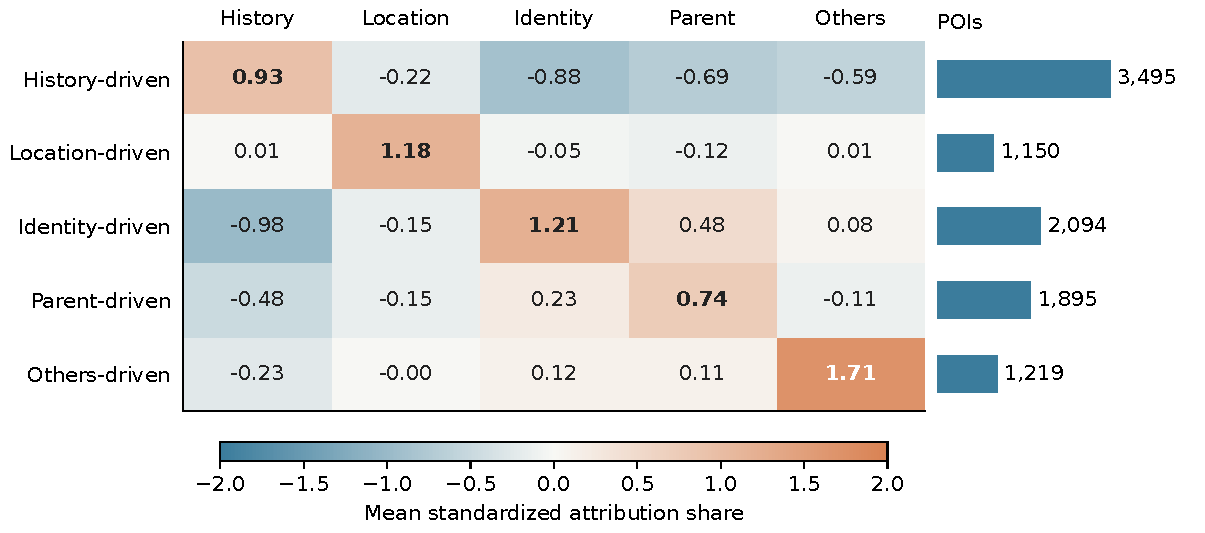
\includegraphics[scale=0.70]{art/attribution_fingerprint.pdf}
\caption{Mean standardized attribution shares and POI counts for the December five-seed consensus at \(T=14\), \(H=7\). Bold values identify the source defining each regime.}
\label{fig:attribution_fingerprint}
\end{figure}

\begin{table}[!htbp]
\centering
\begingroup
\singlespacing
\fontsize{9pt}{10.5pt}\selectfont
\setlength{\tabcolsep}{4pt}
\renewcommand{\arraystretch}{1.08}
\caption{December attribution regimes obtained from the five-seed consensus at $T=14$, $H=7$. Recorded parent counts POIs with an observed containing-place identifier. MAE averages the absolute errors of each fitted model over the same POIs and all test events.}
\label{tab:attri_regime}
\begin{adjustbox}{max width=\linewidth}
\begin{tabular}{lrrr}
\toprule
Regime & POIs & Recorded parent & MAE \\
\midrule
History-driven & 3,495 & 259 & 1.460 \\
Location-driven & 1,150 & 46 & 1.527 \\
Identity-driven & 2,094 & 132 & 1.218 \\
Parent-driven & 1,895 & 0 & 0.964 \\
Others-driven & 1,219 & 144 & 1.329 \\
\bottomrule
\end{tabular}
\end{adjustbox}
\endgroup
\end{table}

\begin{table}[!htbp]
\centering
\begingroup
\singlespacing
\fontsize{9pt}{10.5pt}\selectfont
\setlength{\tabcolsep}{4pt}
\renewcommand{\arraystretch}{1.08}
\caption{December regime shares (\%) within broad POI categories. H, L, I, P, and O denote history-driven, location-driven, identity-driven, parent-driven, and others-driven, respectively. Shares use assigned POIs; MAE uses all POIs in the category.}
\label{tab:category_regime_mae}
\begin{adjustbox}{max width=\linewidth}
\begin{tabular}{lrrrrrrr}
\toprule
POI category & POIs & H & L & I & P & O & MAE \\
\midrule
Schools, campuses, and education-related POIs & 294 & 45.1 & 22.2 & 1.7 & 19.5 & 11.6 & 1.237 \\
Repair, towing, and irregular services & 283 & 58.5 & 13.5 & 4.3 & 14.2 & 9.6 & 0.807 \\
Restaurants and cafes & 2,604 & 14.4 & 6.0 & 59.8 & 7.2 & 12.5 & 1.372 \\
Shopping centers and office-building POIs & 2,879 & 39.0 & 14.6 & 6.7 & 26.6 & 13.0 & 1.298 \\
Clinics and medical services & 1,090 & 59.4 & 12.1 & 4.4 & 15.5 & 8.7 & 1.312 \\
Pharmacies and health-related retail & 240 & 27.5 & 15.8 & 8.8 & 26.7 & 21.2 & 1.399 \\
Small local businesses & 1,688 & 45.5 & 13.7 & 4.5 & 27.6 & 8.7 & 1.302 \\
Bars and nightlife POIs & 383 & 14.9 & 3.9 & 37.7 & 22.5 & 20.9 & 1.020 \\
Grocery and daily retail & 423 & 41.6 & 13.4 & 9.3 & 15.1 & 20.6 & 1.425 \\
\bottomrule
\end{tabular}
\end{adjustbox}
\endgroup
\end{table}


\begin{figure}[!htbp]
\centering
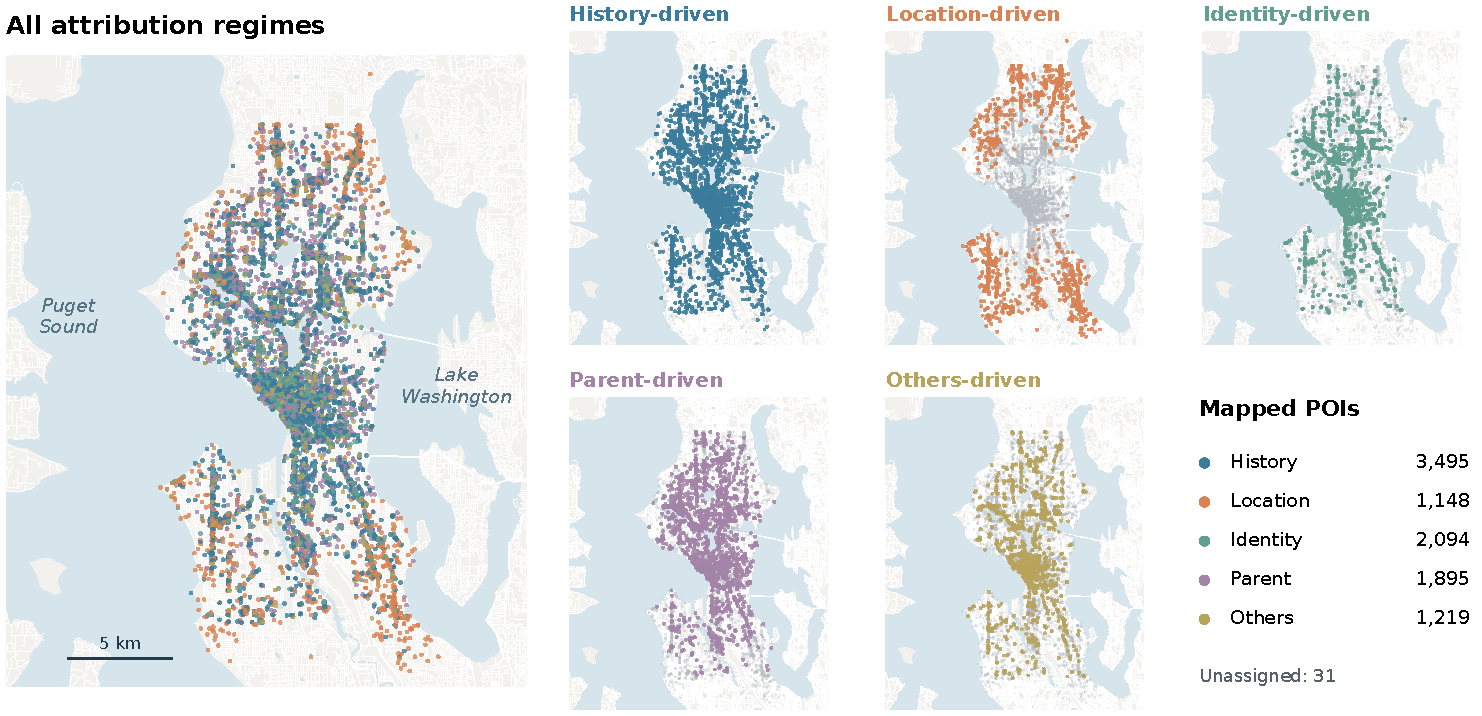
\includegraphics[scale=0.62]{art/attribution_cluster_map.pdf}
\caption{Spatial distribution of the December five-seed attribution consensus. The overview shows all regimes; each small panel highlights one regime against the other POIs. Gray also marks unassigned POIs. Counts refer to the mapped extent. Roads and water are from the 2020 U.S. Census Bureau TIGER/Line files.}
\label{fig:attribution_regime_map}
\end{figure}



\clearpage
\begingroup
\singlespacing
\bibliographystyle{abbrvnat}
\bibliography{reference}
\endgroup

\end{document}
